% This document is part of the transientdict project.
% Copyright 2013 the authors.

\documentclass[12pt]{emulateapj}
\usepackage{graphicx}
\usepackage{subfigure}
%\usepackage{epsfig}
\usepackage{times}
\usepackage{natbib}
\usepackage{amsfonts}
\usepackage{amsmath}
\usepackage{amsbsy}
\usepackage{bm}
\usepackage{hyperref}
%\usepackage[stable]{footmisc}
%\usepackage{color}
%\bibliographystyle{apj}

\newcommand{\project}[1]{\textsl{#1}}
\newcommand{\fermi}{\project{Fermi}}
\newcommand{\rxte}{\project{RXTE}}
\newcommand{\given}{\,|\,}
\newcommand{\dd}{\mathrm{d}}
\newcommand{\counts}{y}
\newcommand{\pars}{\theta}
\newcommand{\mean}{\lambda}
\newcommand{\likelihood}{{\mathcal L}}
\newcommand{\Poisson}{{\mathcal P}}
\newcommand{\Uniform}{{\mathcal U}}
\newcommand{\bg}{\mathrm{bg}}
\newcommand{\word}{\phi}
%\newcommand{\bs}{\boldsymbol}

\begin{document}

\title{Dissecting Magnetar Variability with Probabilistic Generative Models}

\author{D. Huppenkothen\altaffilmark{1, 2}, B. J. Brewer\altaffilmark{}, D. Hogg\altaffilmark{}, I. Murray\altaffilmark{}, M. Frean\altaffilmark{}, C. Elenbaas\altaffilmark{1}, A. L. Watts\altaffilmark{1}, Y.Levin\altaffilmark{}, A.J. van der Horst\altaffilmark{1}, C. Kouveliotou\altaffilmark{3,4}}
 
\altaffiltext{1}{Anton Pannekoek Institute for Astronomy, University of
  Amsterdam, Postbus 94249, 1090 GE Amsterdam, the Netherlands}
  \altaffiltext{2}{Email: D.Huppenkothen@uva.nl}
\altaffiltext{3}{Astrophysics Office, ZP 12, NASA-Marshall Space Flight Center, Huntsville, AL 35812, USA}
\altaffiltext{4}{NSSTC, 320 Sparkman Drive, Huntsville, AL 35805, USA}
\altaffiltext{}{Department of Statistics, The University of Auckland, Private Bag 92019, Auckland 1142, New Zealand}
\altaffiltext{}{Monash Center for Astrophysics and School of Physics, Monash University, Clayton, Victoria 3800, Australia}


\begin{abstract}
%BJB: We should leave this one in for @OverheardOnAstroph:
%Magnetars are whatever and people need whatever.
%Magnetars produce bursts,
%  each of which appears to be composed of a set of one or more spikes.
%Here we build a probabilistic generative model for the \fermi\ GBM photon data on Magnetar bursts.
%The spikes appear to be somewhat asymmetric
%  (rise looks different from decay),
%  have various amplitudes,
%  but have widths that appear to be similar \emph{within} each burst.
%We model each burst as being composed of a mixture of spikes,
%  where each spike is a scaled, stretched, and shifted version of a universal dimensionless function.
%We perform probabilistic inference with a Poisson likelihood and vague priors to determine
%  the positions, amplitudes, and positions of the spikes,
%  the width of the spikes in each burst,
%  and the shape of the dimensionless spike function.
%The phenomenology of spike multiplicity, shape, and width is discussed.
\end{abstract}

\keywords{pulsars: individual (SGR J1550-5418), stars: magnetic fields, stars: neutron, X-rays: bursts, methods:statistics}

\section{Introduction}

With current and upcoming telescopes monitoring the sky regularly across the entire electromagnetic spectrum, time domain astronomy is emerging as one of the key fields in which major 
new discoveries are being made.  A large fraction of astrophysical sources are known to be variable. The timescales span more than five orders of magnitude: fast oscillations in 
X-ray binaries (XRBs) change over milliseconds \citep[e.g.][]{xrb_khzqpos}, while red giants have been observed to change over decades or even centuries \citep[e.g.][]{dasch_giants}. 
Variability studies have the potential to unravel fundamental physical processes: studying variability in XRBs can help us unravel accretion processes and constrain theories of viscosity and strong gravity. 
Similarly, giant flares from magnetars have the potential to map the neutron star interior via neutron star seismology. 

While much of the variability exhibited for example in XRBs can be characterised and made sense of using standard Fourier methodology, this is not true for an important group of sources: for any transients 
with complex temporal structure that is a superposition of different processes. When attempting to disentangle the individual components (for example, a periodic signal from underlying stochastic variability)
using standard methods, it is possible to introduce systematic errors into inferences made from this type of data. Three examples stand out particularly: solar flares, $\gamma$-ray bursts (GRBs) and magnetar bursts.  All three phenomena are characterised by bursts lasting from $\sim 1/10$ of a second to hundreds of seconds, and a 
complex temporal structure that varies strongly from burst to burst (for an example, see Figure \ref{fig:example_bursts}). 

% BJB: you could mention here that taking the fourier transform, while always
% possible, is only "the right thing to do" if you believe the signal is
% periodic.
Fourier methods fail in particular when the underlying processes contributing to the observed light curve, especially deterministic 
components in combination with stochastic variability, are not well known. In this case,
the statistical distributions in the periodogram are not straightforward to model, thus making inferences about the variability in the source problematic. Conversely, 
it is difficult to postulate a common model applicable to a large sample of light curves of these sources. Any light curve model must be flexible enough to account for differences between bursts. 
At the same time, there is a lack of understanding of the underlying physical processes leading to variability in these bursts to inform a choice of model. Here, we aim to develop a probabilistic 
model for highly variable transient events, based on a decomposition of the light curve into simple shapes, without knowing the number of components in the model a priori. We demonstrate the 
power of this approach on a large sample of magnetar bursts, and, for the first time, connect variability in magnetar bursts to the time scales thought to govern the underlying physics.

\begin{figure*}[htbp]
\begin{center}
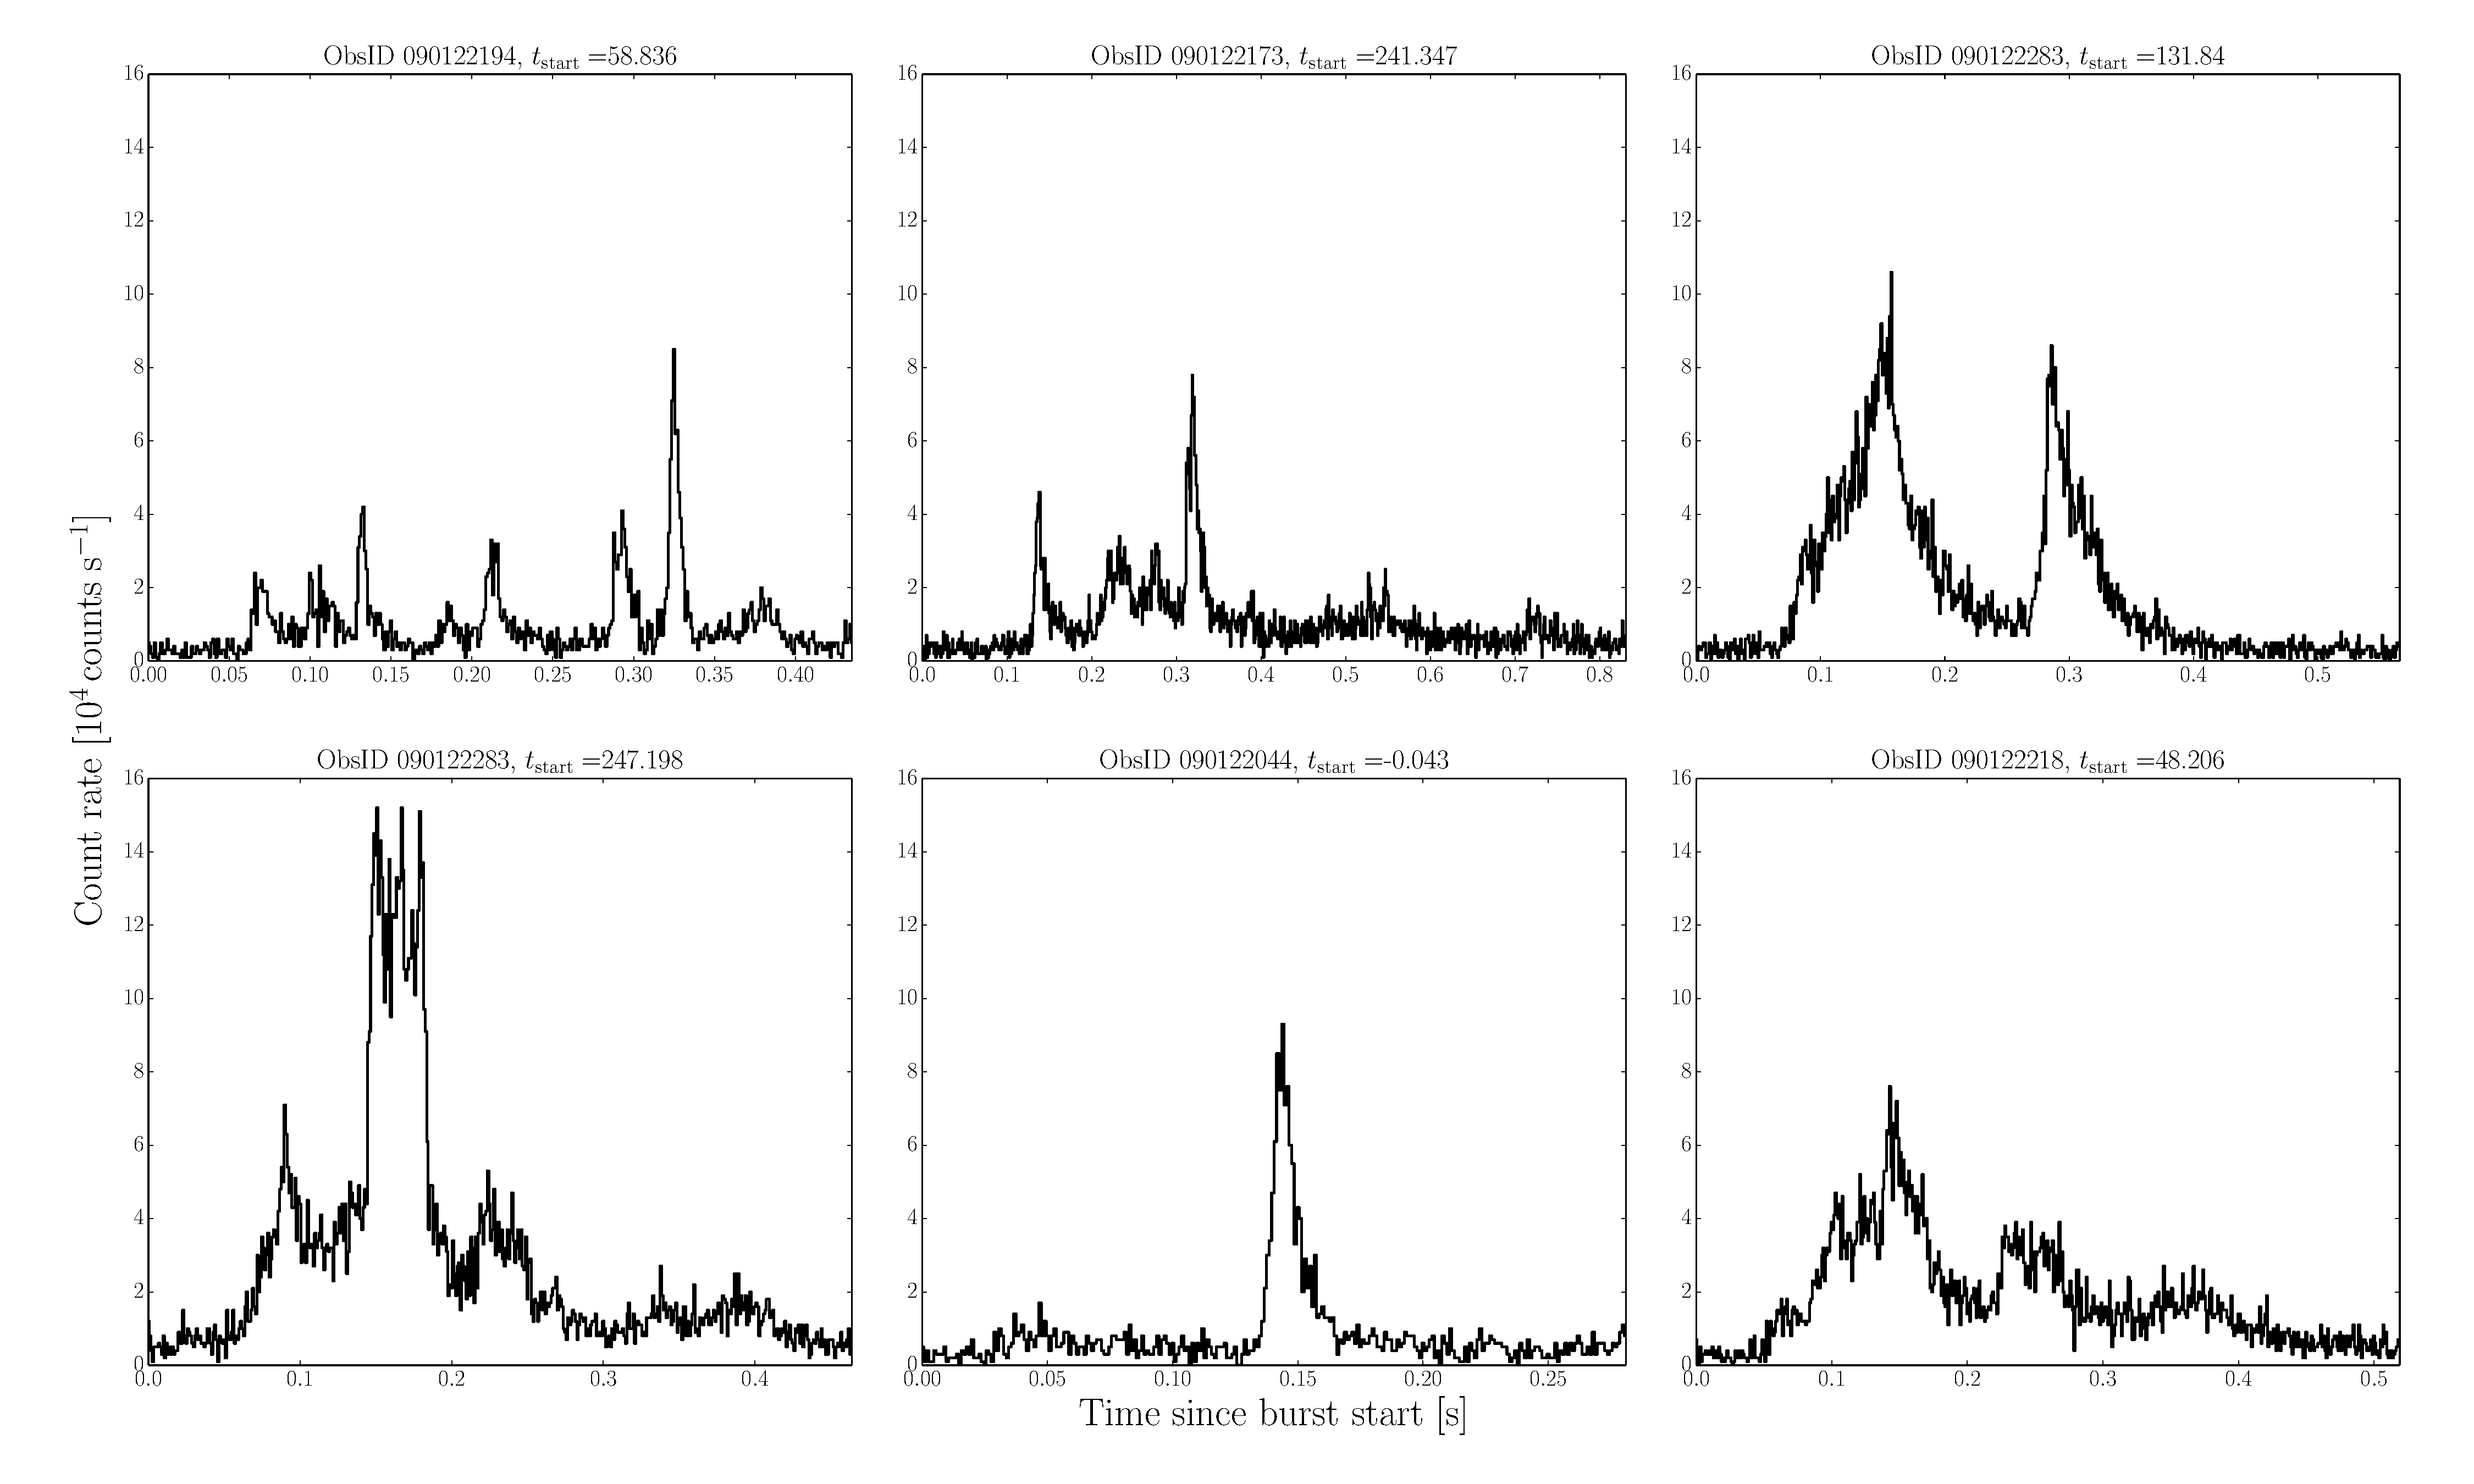
\includegraphics[width=18cm]{example_bursts.pdf}
\caption{Six example bursts observed with \fermi/GBM from the magnetar SGR J1550-5418. Bursts show a complex morphology of one or more
spikes that differs drastically from burst to burst, making development of a common model for all burst light curves difficult. For details on the source
and this sample, see Section \ref{sec:data}.}
\label{fig:example_bursts}
\end{center}
\end{figure*}


Neutron stars, the ultra-dense compact remnants of core-collapse supernovae, are the prime laboratory for studying nuclear 
physical processes in a parameter regime of density and pressure inaccessible to experiments on Earth. 
Among the veritable zoo of neutron star phenomena, two stand out for their peculiar parameters: Soft Gamma Repeaters (SGRs),
named after their hallmark recurring bursts in hard X-rays, and Anomalous X-ray Pulsars (AXPs), persistent pulsating X-ray
sources (taken together, these sources are generally called {\it magnetars}). 

While SGRs and AXPs were detected as separate phenomena, they share common properties \citep[for general overviews of both phenomena, see ][]{woods2006,mereghetti2011}: slow spin periods between
$2 - 12 \, \mathrm{s}$, coupled with generally high period derivatives, lead to large inferred dipole magnetic fields of
the order of $10^{14} \, \mathrm{G}$, well above the quantum-critical limit $B_{\mathrm{QED}} = 4.4 \times 10^{13} \, \mathrm{G}$,
where quantum effects such as pair production and photon splitting become important \citep[although three sources have been 
identified with properties similar to magnetars, but inferred dipole fields below this limit;][]{vanderhorst2010,esposito2010,rea2010,rea2012,scholz2012,rea2014}. 

Both AXPs and SGRs are believed to be the observable phenomena of the same underlying physical system: a highly magnetised
neutron star, also called a magnetar \citep{duncan1992,thompson1995}. In the original scenario, the observable X-ray emission, both persistent emission and bursts, 
is powered by the slow evolution and decay of the source's strong magnetic field, instead of the loss of rotational energy as 
is generally the case for standard radio pulsars \citep{thompson1995,thompson2001}. 

%Magnetar bursts are of particular interest for a variety of reasons. Most importantly, the observation of three giant flares, catastrophic
%outbursts in hard X-rays of energies up to $10^{47} \, \mathrm{erg}$\citep[e.g.][]{mazets1979,cline1998,hurley1999,feroci1999,palmer2005,hurley2004,hurley2005, borkowski2004, mereghetti2005,mazets2005,yamazaki2005,terasawa2005}.% and the associated detection of quasi-periodic oscillations (QPOs)
%in the tails of these flares \citep{israel2005,strohmayer2005,strohmayer2006,watts2006}, have opened up a potential new way to look into the neutron star interior via asteroseismology. 
%In the original model, these giant flares are caused by a catastrophic re-ordering of the neutron star's internal field. As the magnetic field lines, frozen into
%the solid crust, move, the crust responds by fracturing when its breaking strain is exceeded by the forces exerted by the magnetic field.
%The energy released in this process is both released into the magnetosphere, where it forms a pair plasma that slowly radiates away and
%produces the observed emission.%, as well as seismic waves throughout the star. The frequencies of the oscillatory modes depend on
%the nuclear physics of the star's crust and core, making them a prime diagnostic for the conditions inside the star.

%The crust quake model of \citet{thompson1995} is not the only viable model
%for the production of magnetar giant flares. \citet{thompson1995} postulated a catastrophic untwisting the internal magnetic field, which leads to mechanical failure of the neutron star crust.
%Alternatively, the internal magnetic field could unwind slowly, allowing the external magnetic field to follow suit without mechanical failure of the crust. 
%A catastrophic energy release could then occur in the magnetosphere itself, facilitated by explosive reconnection \citep{lyutikov2003,lyutikov2006,heyl2005,nakar2005,masada2010,gill2010}. 
%\citet{vanhoven2011} have shown that a giant flare 
%triggered in the magnetosphere could still excite large-scale shear motions in the crust. In this case, the giant flare would precede the crust quake, and not the other way around.
%A second argument for this alternative picture, akin more to solar flares than earthquakes, comes from calculations that indicate that the physical conditions in the crust
%do not allow for mechanical (brittle) failure \citep{jones2003,horowitz2009}. Instead, the crust is more likely to admit ductile failure and plastic deformation \citep{levin2012}.
%[WHAT DOES THIS MEAN FOR TIME SCALES IN BURSTS?]

Magnetar bursts are of particular interest for a variety of reasons. While the most spectacular outbursts are the rare, but extremely energetic giant flares,
magnetars also show a complex behaviour of emitting much smaller, shorter recurrent bursts. These bursts are of the order of $<1\mathrm{s}$ long, with energies
generally between $10^{38}\,\mathrm{erg}$ and $10^{41}\,\mathrm{erg}$, and have a complex temporal structure with single or
multiple peaks that differs from one burst to the next. They are observed either appearing individually, or in burst 
storms, where tens or hundreds of bursts can occur over a timescale of single days to weeks\citep{mazets1999,goetz2006b,israel2008,mereghetti2009,savchenko2010,israel2010,scholz2011,dib2012,vanderhorst2012,vonkienlin2012}. 
The appearance of bursts appears to be random\citep{gogus1999,gogus2000}, but far more numerous than the giant flares: 
for the two best-observed magnetars, SGR 1806-20 and SGR 1900+14, the
data set spans thousands of such bursts. 

One observation of particular interest concerns the overall distributions of these bursts: the differential distribution of fluence (integrated flux) and 
the cumulative distribution of waiting times are similar to those observed in earth quakes and solar flares\citep{cheng1996}. Especially the fluence distribution
can be well-modelled by a power law with a power-law index of $\sim 1.7$, believed to be a typical signature for a system obeying 
self-organised criticality (SOC; \citealp{bak1987,bak1988}; for a recent introduction and review on SOC in astrophysics see \citealp{aschwanden2014}.). 
In the SOC framework, the physical system in question continuously drives itself towards a critical state,
without requiring fine tuning. When the critical state is reached, relaxation occurs via a catastrophic release of energy. The system returns
to a subcritical state, and the cycle begins anew. %The standard example of an SOC system is a sand pile: as sand grains are slowly dropped onto
%the pile, the slope of the sand pile steepens gradually. However, there is a critical slope, at which the sand pile can no longer support the 
%additional grains dropped onto it, and relaxation occurs via an avalanche, returning the slope to a sub-critical state. 
One advantage of describing a system in the SOC framework is that while the details of the process leading to the critical state and subsequent
relaxation depend on the physical processes specific to the system, many of the overall statistical properties are universal.

At present, it is not clear whether magnetar bursts are smaller-scale versions of the processes believed to produce a giant flare:
either a rapid rupturing of the neutron star due to an internal re-structuring of the magnetic field, with the energy of the cracking process
released in the magnetosphere, or a slow untwisting of the magnetic field leading to ductile deformations in the crust and explosive 
reconnection in the magnetosphere.
%or perhaps entirely magnetospheric events. In the latter scenario, the evolution of the magnetic field would operate on timescales
%slow enough for the crust to respond with plastic deformation rather than brittle fracture, and the energy release would proceed via
%explosive reconnection in the magnetosphere instead.

%%% do these models predict different timescales, and can we say something here about distinguishing them?

Because of the bursts' complex temporal morphology, differing from burst to burst, it is difficult to extract information from their temporal evolution. 
Many bursts show a pattern of one or multiple spikes, where these spikes sometimes sit on top of each other. To extract parameters that could be related
to physical quantities such as the rise time of each spike and the waiting time distribution between spikes, we need to be able to both determine the 
number of spikes per burst as well as the individual parameters of each spike: this requires efficient sampling over a large parameter space.
At the same time, this process needs to operate automatically without the user's intervention, both to avoid biases introduced by manual fitting, as well as
 to allow for an analysis of the large numbers of magnetar bursts observed from various sources.

% BJB: Better to go gently here by saying inference first, then MCMC, and worry about DNest later (it's too scary and many readers
% would rather understand the modelling ideas and care less about the computation).
In this paper, we propose a new method to model magnetar bursts as a linear combination of simple shapes. Both the number of components
per burst as well as the model parameters for each components are free parameters, to be inferred from the data (in practice, using
Markov Chain Monte Carlo [MCMC]).
We apply this model to a large data set of bursts from SGR J1550-5418, observed with the Gamma-ray Burst Monitor (GBM) on board the \fermi spacecraft.
The high sensitivity of the instrument as well as 
the large number of observed bursts make this source an excellent target to demonstrate the power of the proposed methods. For the first time, 
we extract a wealth of physically relevant time scales from SGR bursts. 
We place these timescales in the context of the SOC framework, and tie them to physical parameters in the system.


%Magnetars make bursts.
%Magnetar bursts have many spikes each.
%The spikes look similar within each burst.
%That motivates a very simple model,
%  in which each burst is made up of a sum of spike models, which we call words.

\section{The Burst Sample}
\label{sec:data}

SGR J1550-5418 (also 1E 1547.0-5408) was first observed with the {\it Einstein} X-ray observatory \citep{lamb1981}
and subsequently classified as an AXP based on its soft X-ray spectrum and possible association with a supernova remnant \citep{gelfand2007}.
%A radio detection of pulsations with a slow spin period of $P = 2.096\mathrm{s}$ and a spin-down of $\dot{P} = 2.318 \times 10^{-14}$, implying a magnetic field of $3.2 \times 10^{14} \, \mathrm{G}$ \citep{camilo2007}, confirmed its classification as a magnetar.

In 2008 and 2009, SGR J1550-5418 exhibited three major bursting episodes (October 2008, January 2009 and March/April 2009), where the 2009 January episode is of special interest as a
burst storm. Hundreds of bursts were observed within a single day with various X-ray telescopes ({\it Swift} Burst Alert Telescope (BAT), \citealp{israel2010, scholz2011}); the \fermi Gamma-Ray Burst Monitor (GBM), \citealp{kaneko2010,vonkienlin2012,vanderhorst2012}; the {\it Rossi X-ray Timing Explorer} (RXTE), \citep{dib2012}, and two main instruments on board the {\it INTEGRAL} spacecraft \citealp{mereghetti2009, savchenko2010})
 
Here, we use a sample of bursts observed with {\it Fermi}/GBM during all three bursting episodes. Bursts from SGR J1550-5418 triggered \fermi/GBM for a total of $126$ 
times between 2008 October 3 and 2009 April 17, with $\sim 450$ bursts observed on its most active day, 2009 January 22, alone. 
Each trigger records data from $30\,\mathrm{s}$ before each trigger to $300\,\mathrm{s}$ after each trigger, upon which the instrument cannot trigger for another $\sim 300 \,\mathrm{s}$. 
After GBM is triggered, subsequent bursts within this time span do not trigger the instrument, but can be found in an untriggered burst search. The resulting data stream consists of 
the arrival times of individual photons (time-tagged events, TTE), with an intrinsic time resolution of $\sim 2\mu\mathrm{s}$, sufficient for probing variability to very short time scales.
We use data from the $12$ NaI detectors, whose energy range of $8$ keV to $4$ MeV is sufficient, since SGR bursts rarely exhibit radiation above $200$ keV. Additionally, we only used detectors with viewing angles to the source $< 60^{\circ}$, and checked whether the source was occulted by the spacecraft and the other instrument, the Large Area Detector (LAT). We use the combined samples of bursts from \citet{vonkienlin2012} and \citet{vanderhorst2012}, and include a total of $332$ bursts in our analysis.
We extracted TTE data between $8 \, \mathrm{keV}$ and $200 \, \mathrm{keV}$ around each burst, starting at $t_{\mathrm{start}} - 0.1 \times\mathrm{T}90$ (the burst duration, $\mathrm{T}90$, is defined as the time in which the central $90\%$ of the photons, starting at $5\%$ and ending at $95\%$, reach the detector) and ending at $t_{\mathrm{start}} + 1.1\times\mathrm{T}90$ in order to ensure the entire burst is within our data set. Photon arrival times are barycentered, i.e. projected to the centre of mass of the solar system, to account for the effects of the relative motion of the space craft and the Earth.

We use light curves with a time resolution of $0.5\,\mathrm{ms}$. The time resolution is chosen small enough to preserve features
in the data on short time scales, while at the same time have a reasonable number of counts per time bin. 

The data is affected by both dead time and saturation. 
Dead time occurs because the instrument cannot record a second photon within $2.6\mu\mathrm{s}$ of arrival of a previous photon. 
The second photon is thus either not recorded at all, or, on occasion, recorded as a single photon with the combined energy. This effectively 
imposes a time scale onto the data, which means that the data then deviate away from the expected Poisson distribution. 
Dead time is harder to quantify and account for than saturation. It is possible to correct count rates based on simulations of the instrument (REF, Bhat et al, 2013),
but this will not correct the statistical distributions. We currently do not take dead time into account in our analysis. 

In addition to dead time, saturation may significantly alter the shape of the arriving bursts. Saturation occurs when the number of arriving photons per second
measured in a single GBM detector exceed the maximum data throughput rate of the science data bus. In this case, transmitted rates are capped at a 
count rate of $3.5 \times 10^{5} \, \mathrm{photons} \; \mathrm{s}^{-1}$, any photons exceeding that number are lost. For very bright bursts, this leads
to a flat-topped spikes truncated at the maximum count rate. Any bursts with count rates this high are excluded from the sample, as the model we
consider is not designed to represent these features. 

We use light curves with a time resolution of $0.5\,\mathrm{ms}$. The time resolution is chosen small enough to preserve features
in the data on short time scales, while at the same time have a reasonable number of counts per time bin. 
Burst durations are defined in $T_{90}$, the time in which $90\%$ of photons arrive at the detector, with $0.2T_{90}$ added on either side
to make sure the entire burst is included. 

%Data for the strongest-field magnetars SGR 1806-20 and SGR 1900+14 are recorded with the {\it Rossi} X-ray Timing Explorer (\RXTE), which someone
%else will write the details about (but data are still time-tagged photon events and suffer from saturation and dead time). 

%In what follows, the data for one burst are photon counts $\counts_n$ (integer) in $N$ bins $n$.
%The data from a few example bursts are shown in Figure \ref{fig:example_bursts}.


\section{Analysis Methods}
\label{sec:methods}
% BJB: Some minor wording changes in the following paragraph
In order to successfully model the complex temporal variability in magnetar bursts, any modelling procedure must satisfy the following criteria: (1) it must be flexible enough to be applicable to a large number of bursts with distinctly different morphologies. We achieve this by decomposing magnetar burst light curves into one or more components with simple shapes, which, taken together, make up a burst. (2) The procedure must be largely automated, and be capable of inferring both the number of components as well as the model parameters for each component without human intervention. The latter is achieved by setting up a Bayesian model, where the number of components is a parameter to be inferred together with the corresponding parameters of the individual components. We use MCMC (particularly, diffusive nested sampling as implemented in DNest \citep{brewer2011}) to sample the posterior distribution over all parameters including the number of components. From samples of the posterior distribution,
we can then study the properties of individual burst components, as well as their properties for a given burst.

\subsection{A Bayesian model for magnetar burst light curves}
\label{sec:model}

For a light curve with $K$ Poisson-distributed counts $\bm{\counts} = \{\counts_k\}$, we define a model as a superposition of $N$ individual components:

% BJB: The parentheses in the equation annoyed me so I added \left and \right
%The model for the data in or near one burst is
\begin{eqnarray}
%p(\counts_n\given\pars) &=& \Poisson(\counts_n\given\mean_n)
%\\
\mean_n &=& \mean_{\bg} + \sum_{n=1}^N \mean_{nk}
\\
\mean_{nk} &\equiv& \int_{t_n-\Delta t/2}^{t_n+\Delta t/2} A_n\,\word\left(\frac{t'-t_n}{\tau}\right)\,\dd t' \; ,
%\begin{equation}
%\word(\xi) &=& \left\{\begin{array}{ll}\exp(\xi) & \mbox{for $\xi<0$}\\ \exp(-\xi/s) & \mbox{for $\xi\geq 0$}\end{array}\right. \, ,
%\end{equation}
\end{eqnarray}

where $\mean_{nk}$ is the mean count rate of the $n^{\mathrm{th}}$ model component in time bin $k$, 
$\mean_{bg}$ is the background count rate of that bin,
and the mean count rate $\mean_{nk}$ in a bin $n$ is defined as the integral over a functional form defining the shape of
the model component $\word$ over the the width of that time bin. The component $\word$ is a generic shape,
and can be modified by an amplitude parameter $A_n$ and a parameter setting the width $\tau_n$, in addition to
parameters such as the time offset $t_n$ and intrinsic parameters further describing the component's shape.
We will define a component model $\word$ for magnetar bursts in Section \ref{sec:wordmodel} below, and
restrict ourselves here to a general description of the model.
 
%where $\Poisson(\counts\given\mean)$ is the Poisson probability of getting count $y$ given mean rate $\mean$,
%  $\pars$ is the vector or blob of all model parameters,
%  $\mean_{\bg}$ is the background (DC) level in the bin,
%  $t_n$ is the time of the center of the bin,
%  $\Delta$ is the full width of the bin,
%  $K$ is the number of words (spikes) $k$ making up the burst,
%  $\phi(\xi)$ is the dimensionless word function,
%  $A_n, t_n$ are the amplitudes and time offsets of the words,
%  and $s, \tau$ set the shape (asymmetry or skew) and rise time of the words.

% BJB: Reworded  
The posterior probability over all model parameters is given by:

\begin{equation}
p(N, \bm{\alpha},\{\bm{\theta}_n \} \given \bm{\counts}, H) = \frac{p(\bm{\counts} \given N, \bm{\alpha}, \{\bm{\theta}_n \}, H) p(N, \bm{\alpha}, \{\bm{\theta}_n \} \given H)}{p(\bm{\counts} | H)} \, .
\end{equation}

% BJB: The words "hierarchical model" should appear somewhere around here, but
% I didn't insert them. Might want to define interim prior as p(thetas | alphas, N, H)
Here, $N$ is the number of model components, with the corresponding set of model components $\{\bm{\theta}_n\} = \{ \bm{\theta}_1, \bm{\theta}_2, ..., \bm{\theta}_N \}$. Each $\bm{\theta}_n$ may be a scalar, for models with a single parameter, or a vector.
The scalar or vector $\bm{\alpha}$ encodes the potential hyperparameters used to describe the prior distributions of parameters in $\{\bm{\theta}_n\}$. $H$ encodes the prior choices we have
made about the model that are not part of the inference problem at this stage: for example, the choice of shape for prior distributions and the model shape used to represent the light curve.

We use a Poisson likelihood to describe the data,

\begin{eqnarray}
\likelihood(N, \bm{\alpha}, \{\bm{\theta}_n \}) & = & p(\bm{\counts} \given N, \bm{\alpha}, \{\bm{\theta}_n \}, H) \\ \nonumber
 &= & \prod\limits_{k=0}^{K}{ \frac{e^{-\lambda} \lambda^{y_k} }{y_k! }} \; ,
\end{eqnarray}

which only depends on the parameters of the individual model components, $\{\bm{\theta}_n\}$. In general, the interim priors for the model 
parameters $\{\bm{\theta}_n\}$ will depend on the priors for the hyperparameters defining their prior distributions, $\bm{\alpha}$, such that the
overall prior for this model is

% BJB "Given H" was missing from some of these terms
\begin{equation}
p(N, \bm{\alpha}, \{\bm{\theta}_n \} \given H) = p(N | H)p(\alpha\given N, H)p(\{\bm{\theta}_n\}\given \alpha, N, H) \; .
\end{equation}

Under the assumption that $\bm{\alpha}$ and $N$ are independent, and that the interim priors of the individual model components are
independent and identically distributed, we can re-write this equation as:

% BJB: Fixed mistake in this equation that was caused by me initially (from that RJObject document). Sorry
\begin{equation}
p(N, \bm{\alpha}, \{\bm{\theta}_n \} \given H) = p(N|H)p(\alpha|H) \prod\limits_{n=0}^{N}  p(\bm{\theta}_n\given \alpha, H) \; .
\end{equation}

Thus, the posterior probability density becomes

% BJB: Brackets and H again
\begin{eqnarray}
p(N, \bm{\alpha}, &&\{\bm{\theta}_n \}  \given \bm{\counts}, H) = \\ 
&& \frac{\prod\limits_{k=0}^{K}{ \frac{e^{-\lambda} \lambda^{y_k} }{y_k! }} p(N|H)p(\alpha|H) \prod\limits_{n=0}^{N}  p(\bm{\theta}_n\given \alpha)}{p(\bm{\counts} | H)}  \nonumber
\end{eqnarray}

where the marginal likelihood, $p(\bm{\counts} | H)$ is defined as a normalisation constant in the usual way: 

% BJB: brackets and H again
% BJB: Also, you can't integrate over N as it's discrete :) It's a summation
\begin{eqnarray}
p(\bm{\counts} | H) & = & \sum_{N=0}^{N_{\rm max}} \int_{-\infty}^{\infty}{\likelihood(N, \bm{\alpha}, \{\bm{\theta}_n \})} \times \\ \nonumber
&& p(N|H)p(\alpha|H) \prod\limits_{n=0}^{N}  p(\bm{\theta}_n\given \alpha, H) d\bm{\alpha} d\bm{\theta}_1 ... d\bm{\theta}_N \; .
\label{eqn:marginal}
\end{eqnarray}

The marginal likelihood involves integration in a high-dimensional parameter space as well as summation over $N$, which is analytically intractable for all but the
simplest cases. Here, we use Diffusive Nested Sampling \citep{brewer2011} to efficiently traverse parameter space and approximate the marginal 
likelihood as well as sample from the posterior probability density. 
Nested sampling \citep{skilling2006} samples parameter space by uniformly sampling $M$ points (particles) from the space allowed by the prior. 
One then computes the likelihood values associated with each particle, and the particle with the lowest likelihood is discarded. A new point
can be generated, for example, via Markov Chain Monte Carlo (MCMC), subject to the hard constraint that the
likelihood of the new point must be larger than the likelihood of the discarded one. In this way, the population iterates progressively towards
regions of higher likelihood. At the same time, one may assign a value $X  \in [0, 1]$ to the discarded particle. This effectively provides a 
mapping from parameter space into $[0,1]$, such that the evaluation of the marginal likelihood simplifies to a one-dimensional 
integral tractable with numerical integration methods.

The MCMC step is the key challenge in any Nested Sampling algorithm, and classical MCMC often fails for probability distributions that
are highly multi-modal or contain phase transitions. It is here that Diffusive Nested Sampling provides a reliable alternative \citep[for details, see][]{brewer2011}. 
Instead of recording the end point of an MCMC chain as the new particle, the likelihoods of parameter sets visited during the MCMC exploration step
 are recorded. One can then compute the $1-e^{-1}$ quantile, and record this value as the new likelihood contour, such that the prior space
 under consideration contracts by a factor of $\sim e$. Instead of enforcing a hard likelihood constraint, one now samples a mixture of the 
 two regions, and the particle may escape into the lower-likelihood region, where it can explore more freely. Once enough samples are accumulated,
 one again computes the $1-e^{-1}$ quantile, and constructs a new likelihood contour. This process is repeated, and as in the classical Nested Sampling
 approach, the population contracts towards regions of high likelihood, but it will do so even for complex probability distributions subject to multi-modality
 or phase transitions.

Diffusive nested sampling as implemented in {\it DNest3}\footnote{the code is available under the GNU public license at \hyperref[]{https://github.com/eggplantbren/DNest3}} can return both an estimate for the marginal likelihood,
suitable for model selection purposes, as well as a samples drawn from the posterior probability density function (pdf) for a given burst. The latter is done by letting a particle explore
the final mixture of levels freely via MCMC. 
We can make inferences about individual parameters in the model from these samples in the usual way by marginalising over nuisance parameters (e.g. 
hyper parameters $\bm{\alpha}$). Additionally, for many bursts, we can make inferences over the parameters from many components. In the naive way,
this can be done by picking a parameter set from the MCMC run for each burst, and using this ensemble of individual samples from many bursts 
to compute the quantity of interest (say, a correlation between two model parameters). This procedure can be repeated, such that we build up a sample
for the quantity in question. Note, however, that by posing that individual bursts have no knowledge of each other - we fit the model for each burst separately - 
this imposes a strong prior on this quantity, suggesting that there is, in fact, no correlation present. 

\begin{figure}[h]
\begin{center}
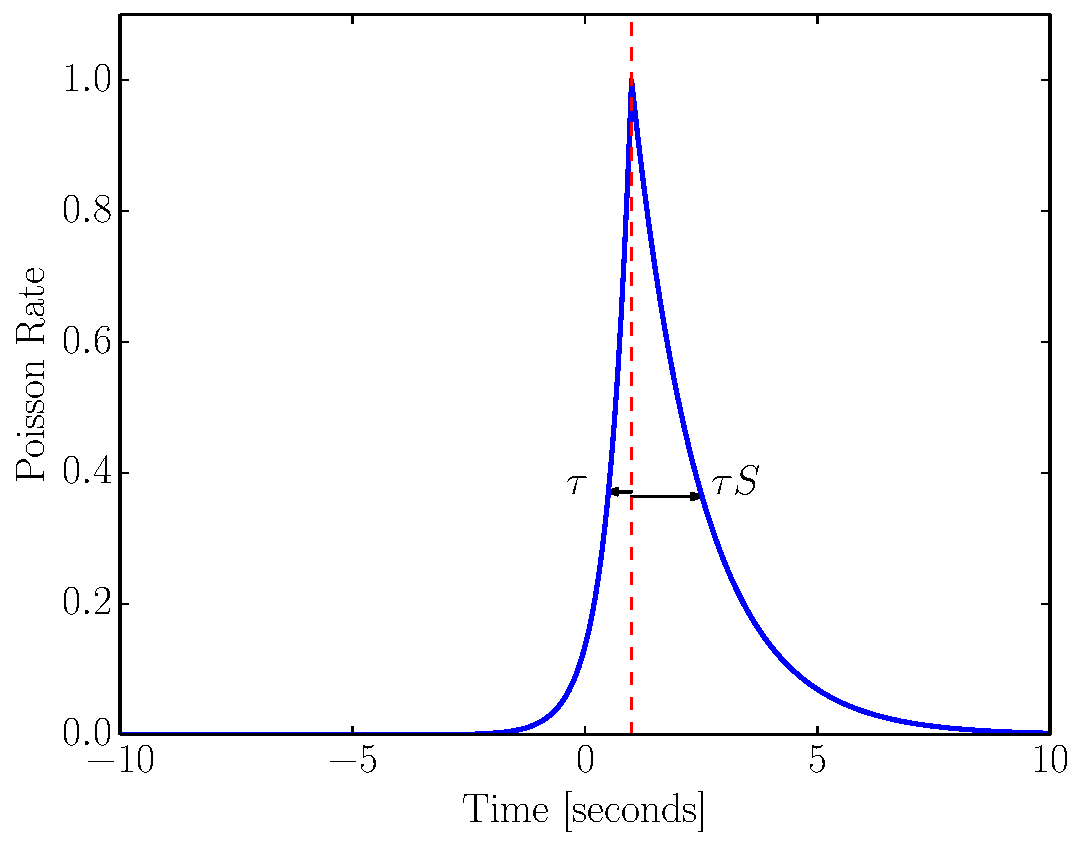
\includegraphics[width=9cm]{word.pdf}
\caption{An example of the component model used for magnetar bursts: a spike is defined by an exponential rise with characteristic
time scale $\tau$ and an exponential fall with a fall time scale $s\tau$, where $s$ is a skewness parameter that describes how the fall
time is stretched ($s > 1$) of contracted ($s < 1$) compared to the rise time. Individual spikes are also characterised by a time offset
$t$ describing the location of the peak count rate in a time series, and an amplitude $A$ describing the height of a peak.}
\label{fig:word_example}
\end{center}
\end{figure}
\subsection{Model shapes}
\label{sec:wordmodel}
For the type of exploratory data analysis considered here, this is sufficient. A formally correct implementation would have to include a Bayesian hierarchical model,
where many bursts are considered in the same model, with appropriate priors on any quantities to be measured across samples of many bursts. This can, in turn,
be extended again to make inferences across, for example, different magnetars. The latter two steps are beyond the scope of this work, but will be explored in the future.



The model defined in Section \ref{sec:model} is fairly general: it is valid for any Poisson-distributed light curve thought to be composed several individual components of
the same shape, but with potentially different individual parameters (such as amplitudes and widths). 
We have made only three assumptions so far: the likelihood follows a Poisson distribution, the priors for the number of components $N$ and the hyper parameters $\bm{\alpha}$ are independent,
and the priors on the parameters of the model for the individual components are independent of each other and identically distributed. 
Here, we now refine this model for magnetar bursts specifically. However, changing the model shape for use with different source classes (e.g. GRBs) is straightforward.

Magnetar bursts are short events composed of one or more sharp, spike-like features (see Figure \ref{fig:example_bursts} for various examples). We model these features
with a sharp spike consisting of an exponential rise and an exponential decay of the type:


%The model for the data in or near one burst is
%\begin{eqnarray}
%p(\counts_n\given\pars) &=& \Poisson(\counts_n\given\mean_n)
%\\
%\mean_n &=& \mean_{\bg} + \sum_{k=1}^K \mean_{nk}
%\\
%\mean_{nk} &\equiv& \int_{t_n-\Delta/2}^{t_n+\Delta/2} A_n\,\word(\frac{t'-t_n}{\tau})\,\dd t'
%\\
\begin{equation}
\word(t) = A \left\{\begin{array}{ll}\exp(t-t_{\mathrm{offset}}/\tau) & \mbox{for $t < t_{\mathrm{offset}}$}\\ 
\exp(-(t-t_{\mathrm{offset}})/(\tau s)) & \mbox{for $t \geq t_\mathrm{offset}$}\end{array}\right. \, ,
\label{eqn:word}
\end{equation}
%\end{eqnarray}

where $\word(ti)$ is the component function depending on time parameter $t$ and a skewness
parameter $s$. By giving each component $n$ in the model a time offset $t_{\mathrm{offset},n}$ (equivalent to the time of the peak), 
an amplitude $A_n$ and an exponential rise timescale $\tau_n$ in addition to the skewness parameter $s_n$, 
these spikes can become a representation of the spikes observed in magnetar burst light curves (see Figure \ref{fig:word_example}
for an example of the model).


For each component $n$, we have a set of free parameters $\{t_n, A_n, \tau_n, s_n \},$, for each model, i.e. each
linear combination of components, we have a set of free parameters $\{\mean_{bg}, \{t_n, A_n, \tau_n, s_n\} \}$.
We set a uniform prior on the number of components $N$, where $N$ may lie between $0$ and $100$. 
The priors for the free parameters of the individual components are independent and identically distributed, such that priors 
are the same for a given type of parameter between components. 
Because bursts are defined in such a way that the observed count rate must drop back to the background before the
start and the end of each burst, we can simply define the prior on the time offset such that $t_n$ must lie between
the start and end times of the burst light curve, $t_{\mathrm{start}} < t_n < t_\mathrm{end}$. 
For the amplitude $A_n$ and the rise timescale $\tau_n$, we choose exponential priors:

\begin{figure*}[htbp]
%\begin{center}
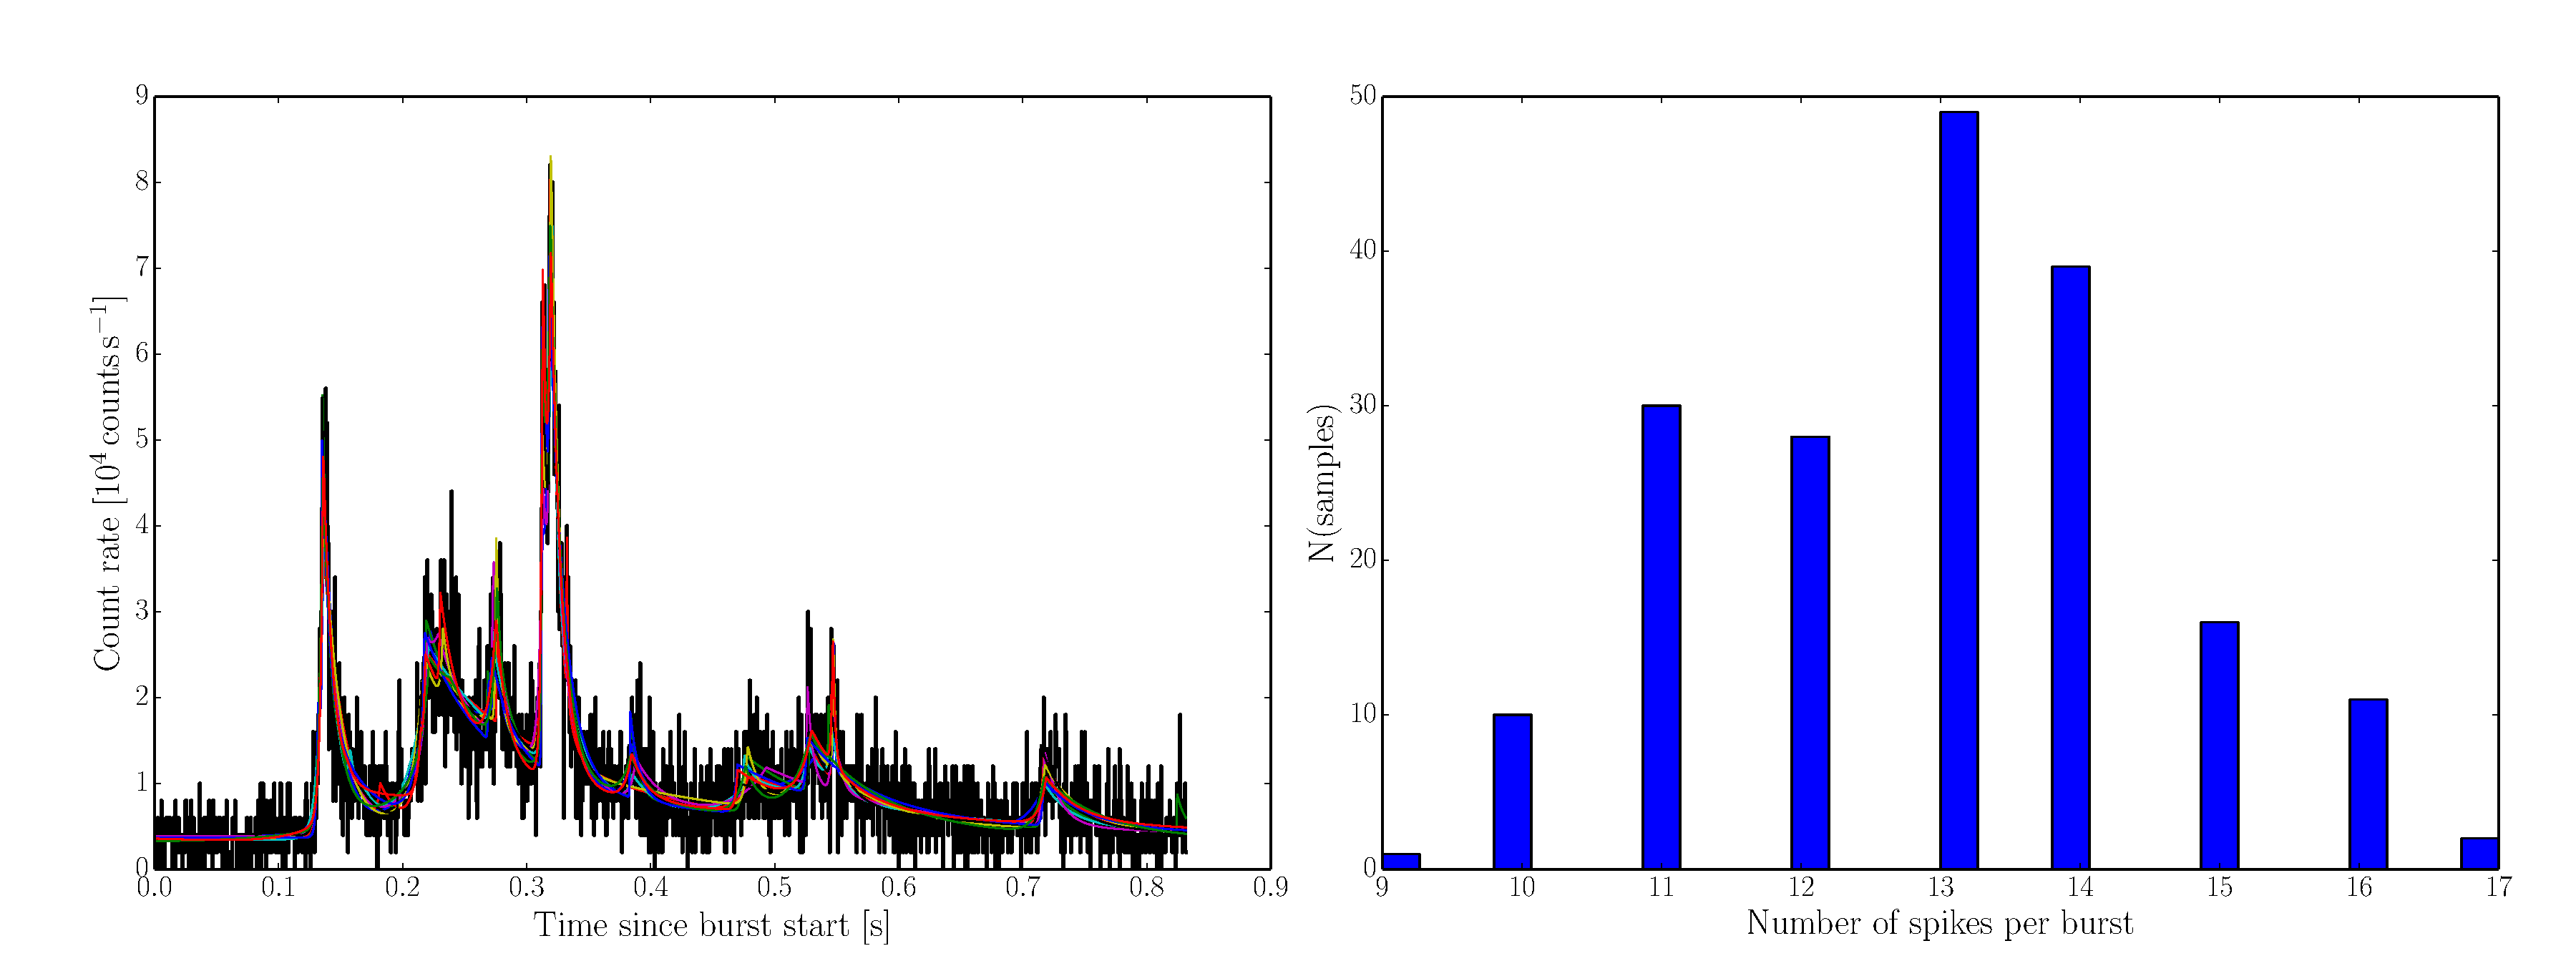
\includegraphics[width=\textwidth]{example_dnest_result.pdf}
\caption{An example burst from the magnetar SGR J1550-5418, in an observation taken on 2009 January 22 (ObsID 090122173). In the left
panel, the light curve at high time resolution, $\Delta t = 5 \times 10^{-4}$, and model light curves for $10$ random draws from the posterior pdf. 
On the right, the marginalised posterior pdf over the possible number of components in the model. The posterior for the number of components is 
quite well constrained between $9$ and $17$ components.}
\label{fig:dnest_example}
%\end{center}
\end{figure*}


\begin{eqnarray}
p(A \given \mu_A) &=& e^{(A/\mu_A)} \\
p(\tau \given \mu_{\tau} & = & e^{(\frac{\tau - \tau_{\mathrm{min}}}{\mu_{\mathrm{\tau}}})} \; ,
\end{eqnarray}

where $\mu_A$ and $\mu_{\mathrm{\tau}}$ are hyper parameters describing the width of the exponential distribution.
We set a minimum possible rise time scale $\tau_{\mathrm{min}}$ to be a fraction of the light curve's time resolution,
$\tau_{\mathrm{min}} = \Delta t/10$: the time resolution effectively limits the information on the rise time we can extract.

The prior on the skewness parameter $s_n$ is a uniform distribution with a mean of $a$ and a half-width of $b$, such
that the log-skewness must lie in the range $(a-b) < \log{(s)} < (a+b)$. A definition in terms of mean and half-width ensures
that positive and negative skews are equally likely a priori.


The prior on the background parameter, finally, depends on the data itself. It is log-uniform, with boundaries between 
$\log{(10^{-3}\mu_\counts)} < \log{(\counts_{\mathrm{bg}})} < \log{(10^{3} \mu_\counts)}$, where $\mu_\counts$ is the average count
rate in a burst. Note that this is, in principle, not a valid prior: the prior for the parameters should not depend on the data
itself. In practice, it is convenient as long as one does not need to compute the marginal likelihood. In a more in-depth analysis
involving the marginal likelihood where, for example, one might test whether any results change with a change of prior, or where different component models
might be compared, one would need to discard this prior for one that is formally valid.

The priors on the hyper parameters $\mu_{A}$ and $\mu_{\mathrm{\tau}}$ are log-uniform. The prior range for
$\mu_{\tau}$ depends on the length of the data set, such that $\log{(10^{-3}t_{\mathrm{burst}})} < \log{(\mu_{\tau})} < \log{(10^{3}t_\mathrm{burst})}$.
Like the prior on the background count rate $\counts_{\mathrm{bg}}$, the hyper prior on the width of the amplitude prior distribution
depends on the count rate in a burst, $\mu_\counts$: $\log{(10^{-3}\mu_\counts)} < \log{(\mu_{A})} < \log{(10^{3} \mu_\counts)}$. The same reasoning applies as
for the background prior, such that for a more complicated analysis involving the marginal likelihood it needs to be replaced
by a prior that is formally valid.

We show an example of a burst light curve, together with random draws from the posterior distribution, in Figure \ref{fig:dnest_example}.



%where $\Poisson(\counts\given\mean)$ is the Poisson probability of getting count $y$ given mean rate $\mean$,
%  $\pars$ is the vector or blob of all model parameters,
%  $\mean_{\bg}$ is the background (DC) level in the bin,
%  $t_n$ is the time of the center of the bin,
%  $\Delta$ is the full width of the bin,
%  $K$ is the number of words (spikes) $k$ making up the burst,
%  $\phi(\xi)$ is the dimensionless word function,
%  $A_n, t_n$ are the amplitudes and time offsets of the words,
%  and $s, \tau$ set the shape (asymmetry or skew) and rise time of the words.
  
%Various parameters can be left free completely, or can be tied together between words:
 
%\begin{equation}
%\theta \equiv [,\{t_n, \tau_n, A_n, s_n \}_{k=1}^K, \mean_{\bg} ]
%\end{equation}

%for complete freedom of word parameters between words,

%\begin{equation}
%\theta \equiv [,\{t_n, A_n, s_n \}_{k=1}^K,  \tau_n, \mean_{\bg} ]
%\end{equation}

%for tying the rise time together within a burst, and

%\begin{equation}
%\theta \equiv [,\{t_n, A_n\}_{k=1}^K, \tau_n, s_n , \mean_{\bg} ]\end{equation}

%for a model where both the rise time and the skewness are tied together for all words within a burst.

%\begin{figure*}[h]
%\begin{center}
%\includegraphics[width=18cm]{example_words.png}
%\caption{}
%\label{fig:example_words}
%\end{center}
%\end{figure*}

  
%Figure \ref{fig:example_words} shows the shape of a word
%  and an example of a burst generated by our model.

%The model for a large set of bursts is whatever.
%[We should probably, in the above, index bursts $m$,
%  and maybe even magnetar $j$.]

%\emph{Notes to selves:}
%At one point we figured we could \emph{fix} shape parameter $s$
%  to be the same for all the words in all the bursts from one magnetar,
%  but permit the duration $\tau$ to vary.
%However, as we worked in our coding session we moved more in the direction
%  of thinking in terms of ``rise time'' $\tau$ and decay time $s\,\tau$.
%It might be better to parameterize that way.
%One possible point of discovery would be that the rise times
%  are fundamental to each magnetar,
%  but decay times vary.
%(For instance.)

%The prior pdfs are
%\begin{eqnarray}
%p(\ln\lambda_{\bg}) &=& \Uniform(\ln\lambda_{\bg}\given a_1, a_2)
%\\
%p(\ln s) &=& \Uniform(\ln s\given a_3, a_4)
%\\
%p(\ln\tau) &=& \Uniform(\ln\tau\given a_5, a_6)
%\\
%p(\ln A_n) &=& \Uniform(\ln A_n\given a_7, a_8)
%\\
%p(t_n) &=& \Uniform(t_n\given a_9, a_{10})
%\quad,
%\end{eqnarray}
%where $\Uniform(x\given a, b)$ is the uniform distribution for $x$ in the range $a<x<b$.

%We use \project{emcee} (CITE) to perform MCMC sampling.
%[We initialize the MCMC walkers how?]

%Finally, there is the issue of how to set the number $K$ of words in each burst.
%We take a ``cross-validation'' approach [take that, BJB],
%  in which we ask what value of $K$ does the best job at making posterior predictions
%  about left-out data.
%[We construct this validation test how?]
%Figure [what figure?] shows an example burst,
%  fit with $K=1$, $2$, $3$, $4$, and $5$ words.
%It also shows the result of the posterior-prediction validation
%  that selects $K=4$ as the best choice for this burst.
\begin{figure}[htbp]
\begin{center}
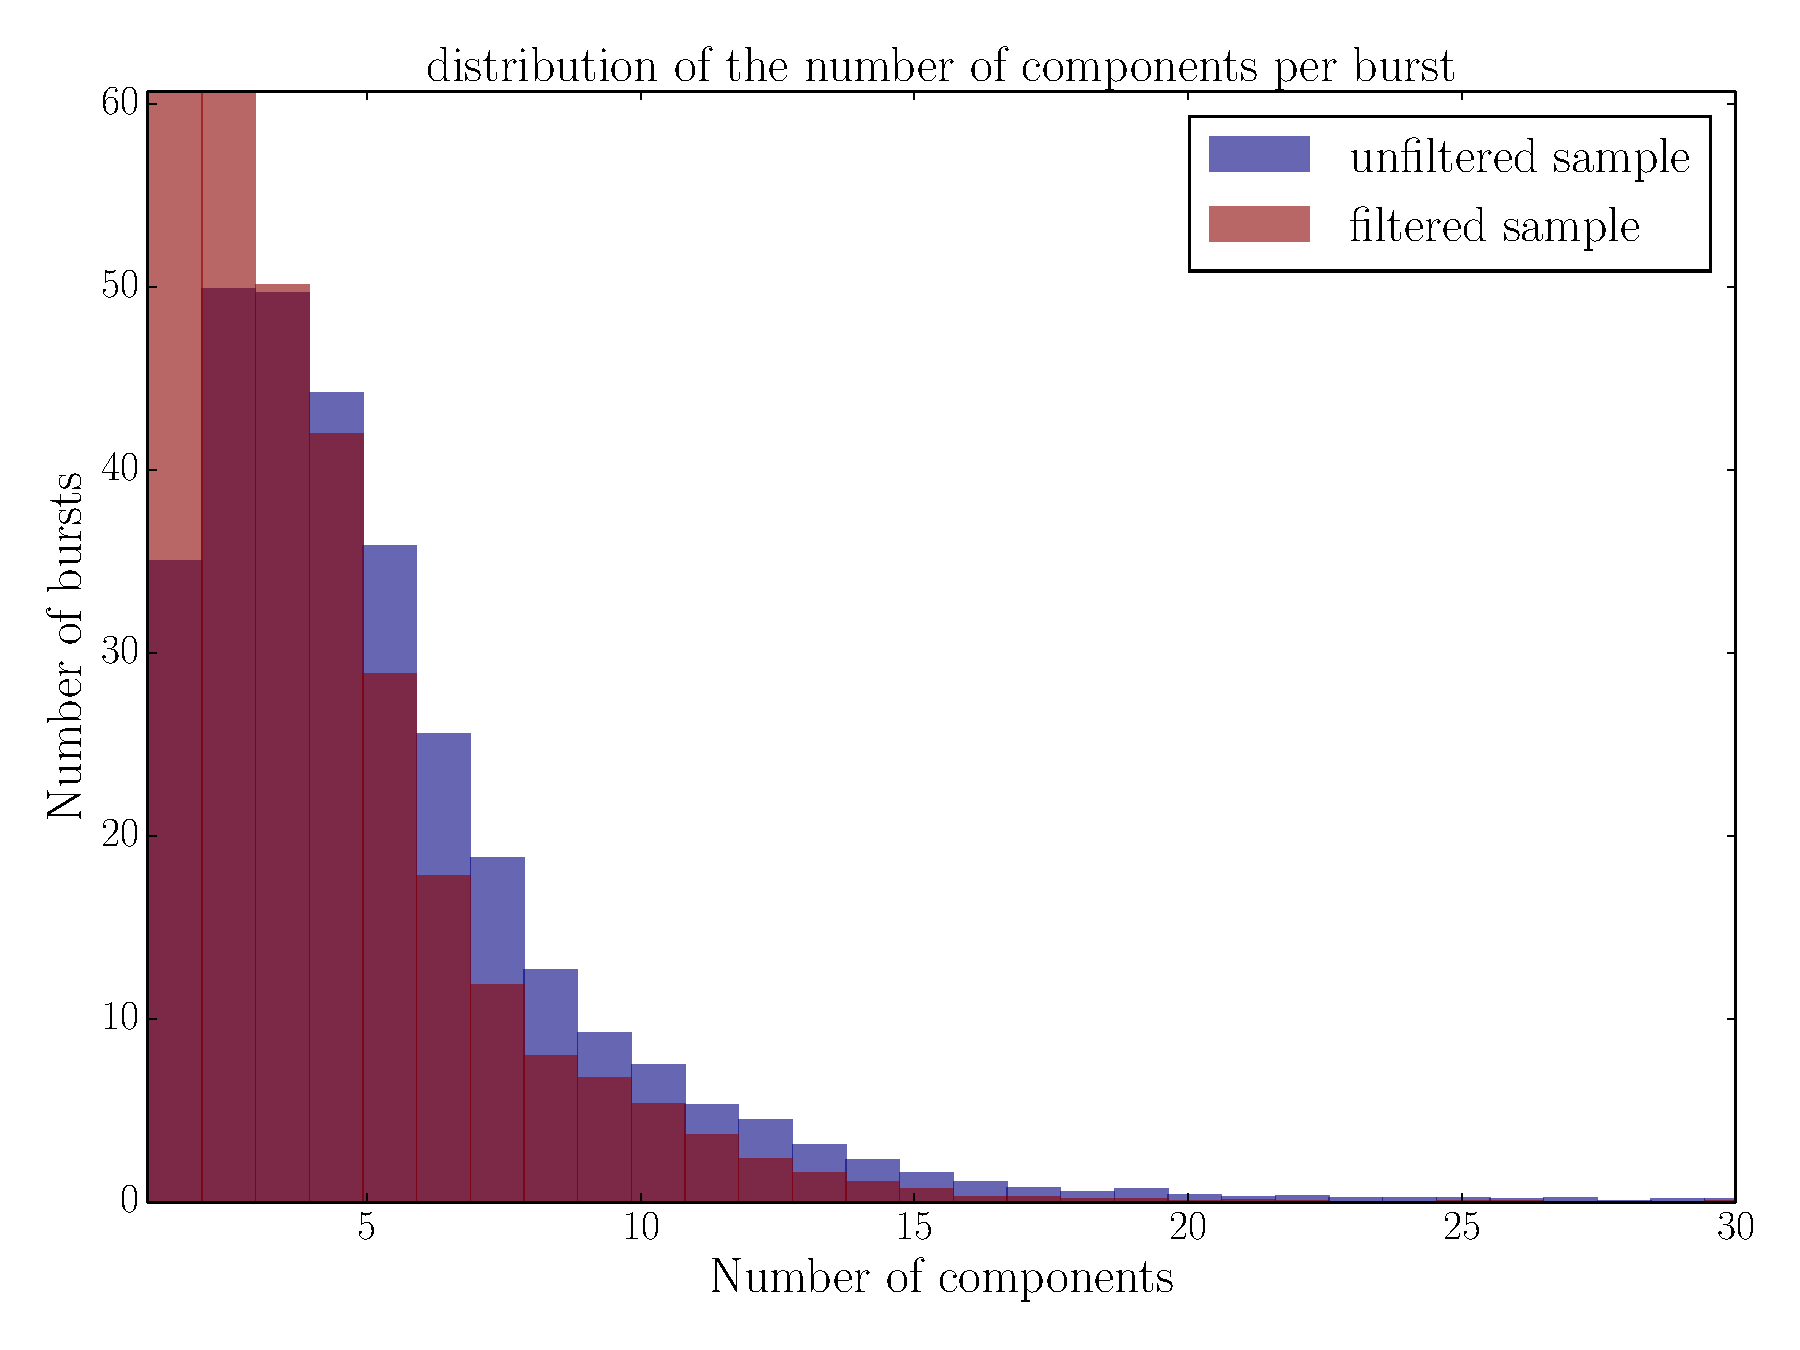
\includegraphics[width=9cm]{sgr1550_nspikes.pdf}
\caption{Number of components in a given burst for $332$ modelled bursts, for both the raw (unfiltered) sample (blue) as
}
\label{fig:spikes}
\end{center}
\end{figure}

\section{Results}

We explored statistical distributions of model parameters, focussing predominantly on the exponential rise time scale $\tau$, 
the amplitude $A$, and as derived quantities the fluence (as a proxy for total dissipated energy) and duration for model spikes for
 the whole {\it Fermi}/GBM sample of bursts from SGR J1550-5418. We sampled from the posterior pdf as approximated in Diffusive 
 Nested sampling, for each individual burst light curve. For inferences across bursts, as mentioned in Section \ref{sec:methods},
this implies a strong prior against any potential correlations between parameters, because we consider the bursts to be separate, independent entities
in this case. Here, we restrict ourselves to simple, qualitative tests, and
leave a full Bayesian hierarchical model with the power to quantify the results presented below to future work. 


\subsection{Exploring Differential Distributions and Correlations Between Key Quantities}
\label{sec:exploration}

A first exploration of the data reveals that most bursts can be represented with only a few spikes, of the order of 
$10$ or less (see also Figure \ref{fig:spikes}). Because we use very high-resolution data for this analysis in order to
be sensitive to short timescales of $< 1\mathrm{ms}$, a primary source for potential biases in our analysis is the
danger that the model might try to represent individual (e.g. background) photons as spike features; this would greatly
skew the resulting distributions towards small amplitudes and very short durations. The fact that we have many bursts
fit with few spikes indicates that this might not be much of a problem. However, we also note that there is an appreciable fraction
of spikes ($\sim 35\%$) with amplitudes smaller than the inferred background count level for the respective model these spikes 
are part of. We cannot say with certainty whether these features are present: they may well be, but the intrinsic sky and instrumental background
 make it difficult to ascertain their presence. Excluding these features from the sample produces a narrower distribution
of spikes per burst, with the maximum clustered at $2$ spikes her bursts (see Figure \ref{fig:spikes}).

In what follows, we exclude spikes with amplitudes smaller than the background count rate. The reason is not that we do not believe
they exist, but rather that their parameters, e.g. their position in time, are largely unconstrained.
This effectively puts a lower limit on the spike amplitudes we consider, which then depends on the instrumental and sky background. We note
that including the smallest features in the analysis does not change our results in a significant way: distributions for 
waiting times and amplitudes have a stronger tail at small waiting times and amplitudes, but their inclusions changes neither
the qualitative behaviour nor the conclusions we draw from this analysis. It would be interesting to explore their possible presence
using bursts observed with an X-ray telescope less affected by sky background than \fermi/GBM is.

\begin{figure*}[htbp]
\begin{center}
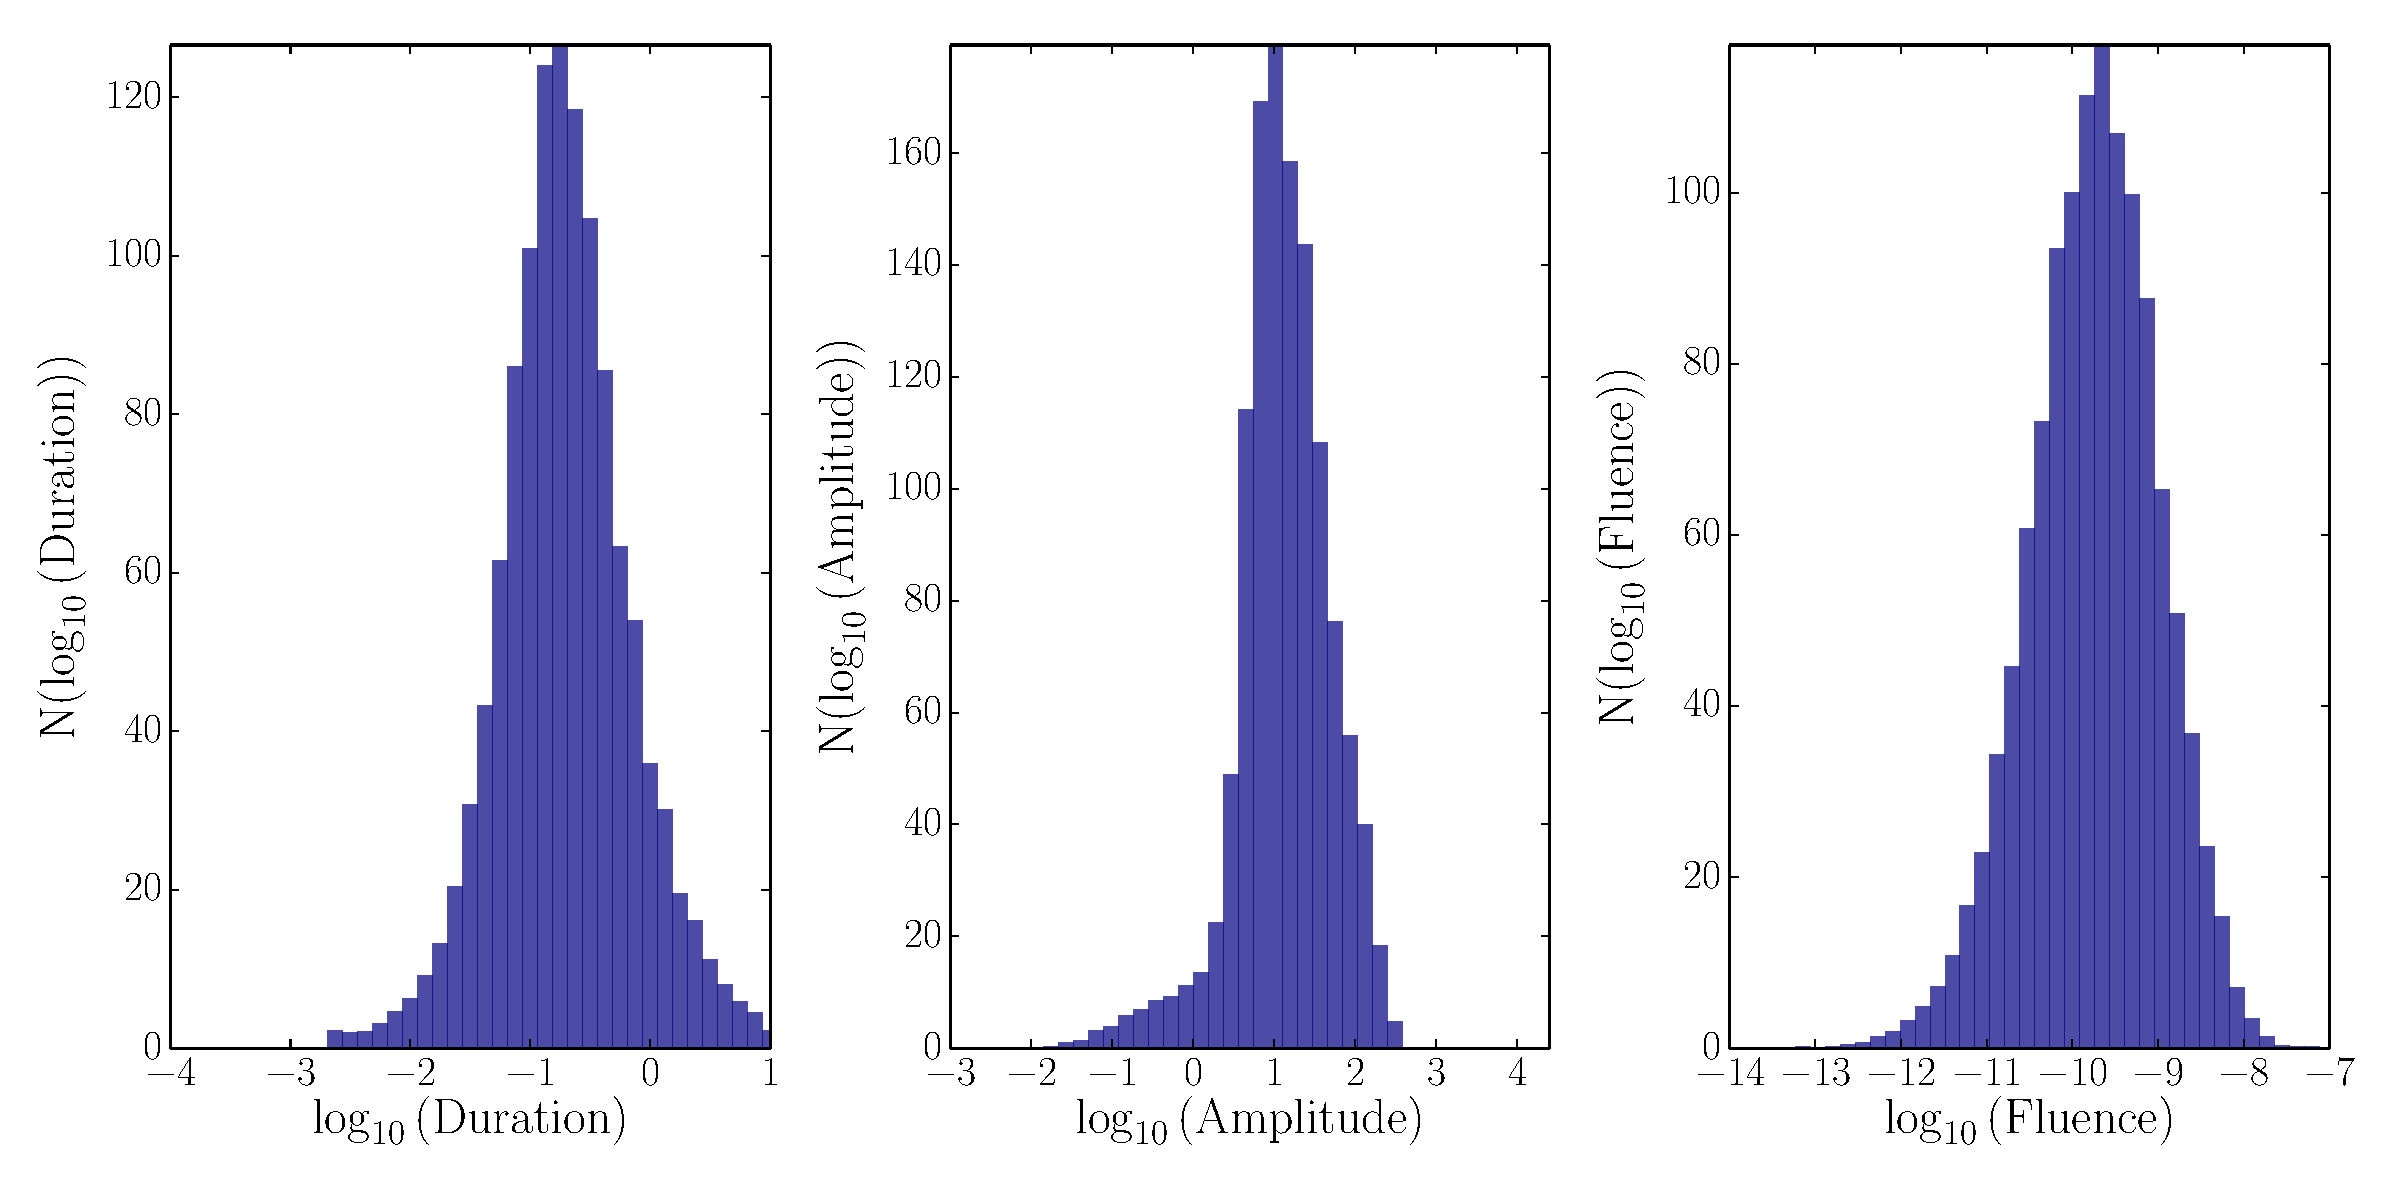
\includegraphics[width=\textwidth]{sgr1550_diff_dist.pdf}
\caption{Differential distributions for the duration, count-space amplitude and fluence for all model components from $332$ bursts. In each bin, we plot the mean for
that bin from $100$ ensembles of random draws from the posterior pdf of each burst (see text for details). All three distributions are strongly peaked and appear slightly 
skewed towards larger values. }
\label{fig:diffdist}
\end{center}
\end{figure*}

Four quantities are of particular interest for their potential connection with physical processes: the spike duration $T$, exponential rise time scale $\tau$,
total dissipated energy $E$ and waiting time between consecutive spikes $t_\mathrm{wait}$. The exponential rise time scale for each model component is a free parameter
in our model, and thus easily extracted. We compute spike duration by finding the time between the two points at which the flux drops by a
 factor of $100$ on either side of the spike peak. Finally, we compute the dissipated energy in a spike by integrating Equation \ref{eqn:word} analytically in count space,
 then converting from count space to fluence using the spectral modelling results from \citet{vanderhorst2012} and \citet{vonkienlin2012}. Because the distance is not well constrained for SGR J1550-5418, we do not convert from fluence to energy, but for a qualitative comparison to the expected correlation between the various quantities, this conversion is irrelevant.
 
 Here, we test for both correlation between fluence and rise time as well as fluence and duration, as well as construct differential distributions
 in order to compare with predictions from SOC theory. We construct differential distributions by picking a sample from the posterior distribution
 for each burst in the data set, and hence form an ensemble of posterior draws for all bursts, for which we can construct the differential distribution.
 We repeat this process $S$ times, such that we have $S$ ensembles of burst models and $S$ differential distributions, and plot the mean of the distribution in
 each bin of that distribution. 
 Similarly, we test for correlations by $S$ ensembles of burst models and testing for the presence of a correlation using a Spearman rank
 coefficient for each ensemble. We then report the mean and standard deviation of the distribution of coefficients for $S$ draws, where $S = 100$ in all cases below.
 
 
 In Figure \ref{fig:diffdist}, we show differential distributions of duration, peak amplitude (measured in count space) and fluence for all spikes in $332$ bursts. All three distributions are
 strongly peaked, and both amplitude and fluence are skewed towards larger values. The latter is exacerbated when considering the unfiltered sample of 
 spikes (including spikes with peak amplitudes below the background count rate), producing longer tails for both amplitude and fluence, but not changing the qualitative behaviour of the distributions. We will consider the behaviour of
 the differential distributions in detail and compare the observed distributions to predictions from SOC theory in Section \ref{sec:soc}.

 \begin{figure}[htbp]
\begin{center}
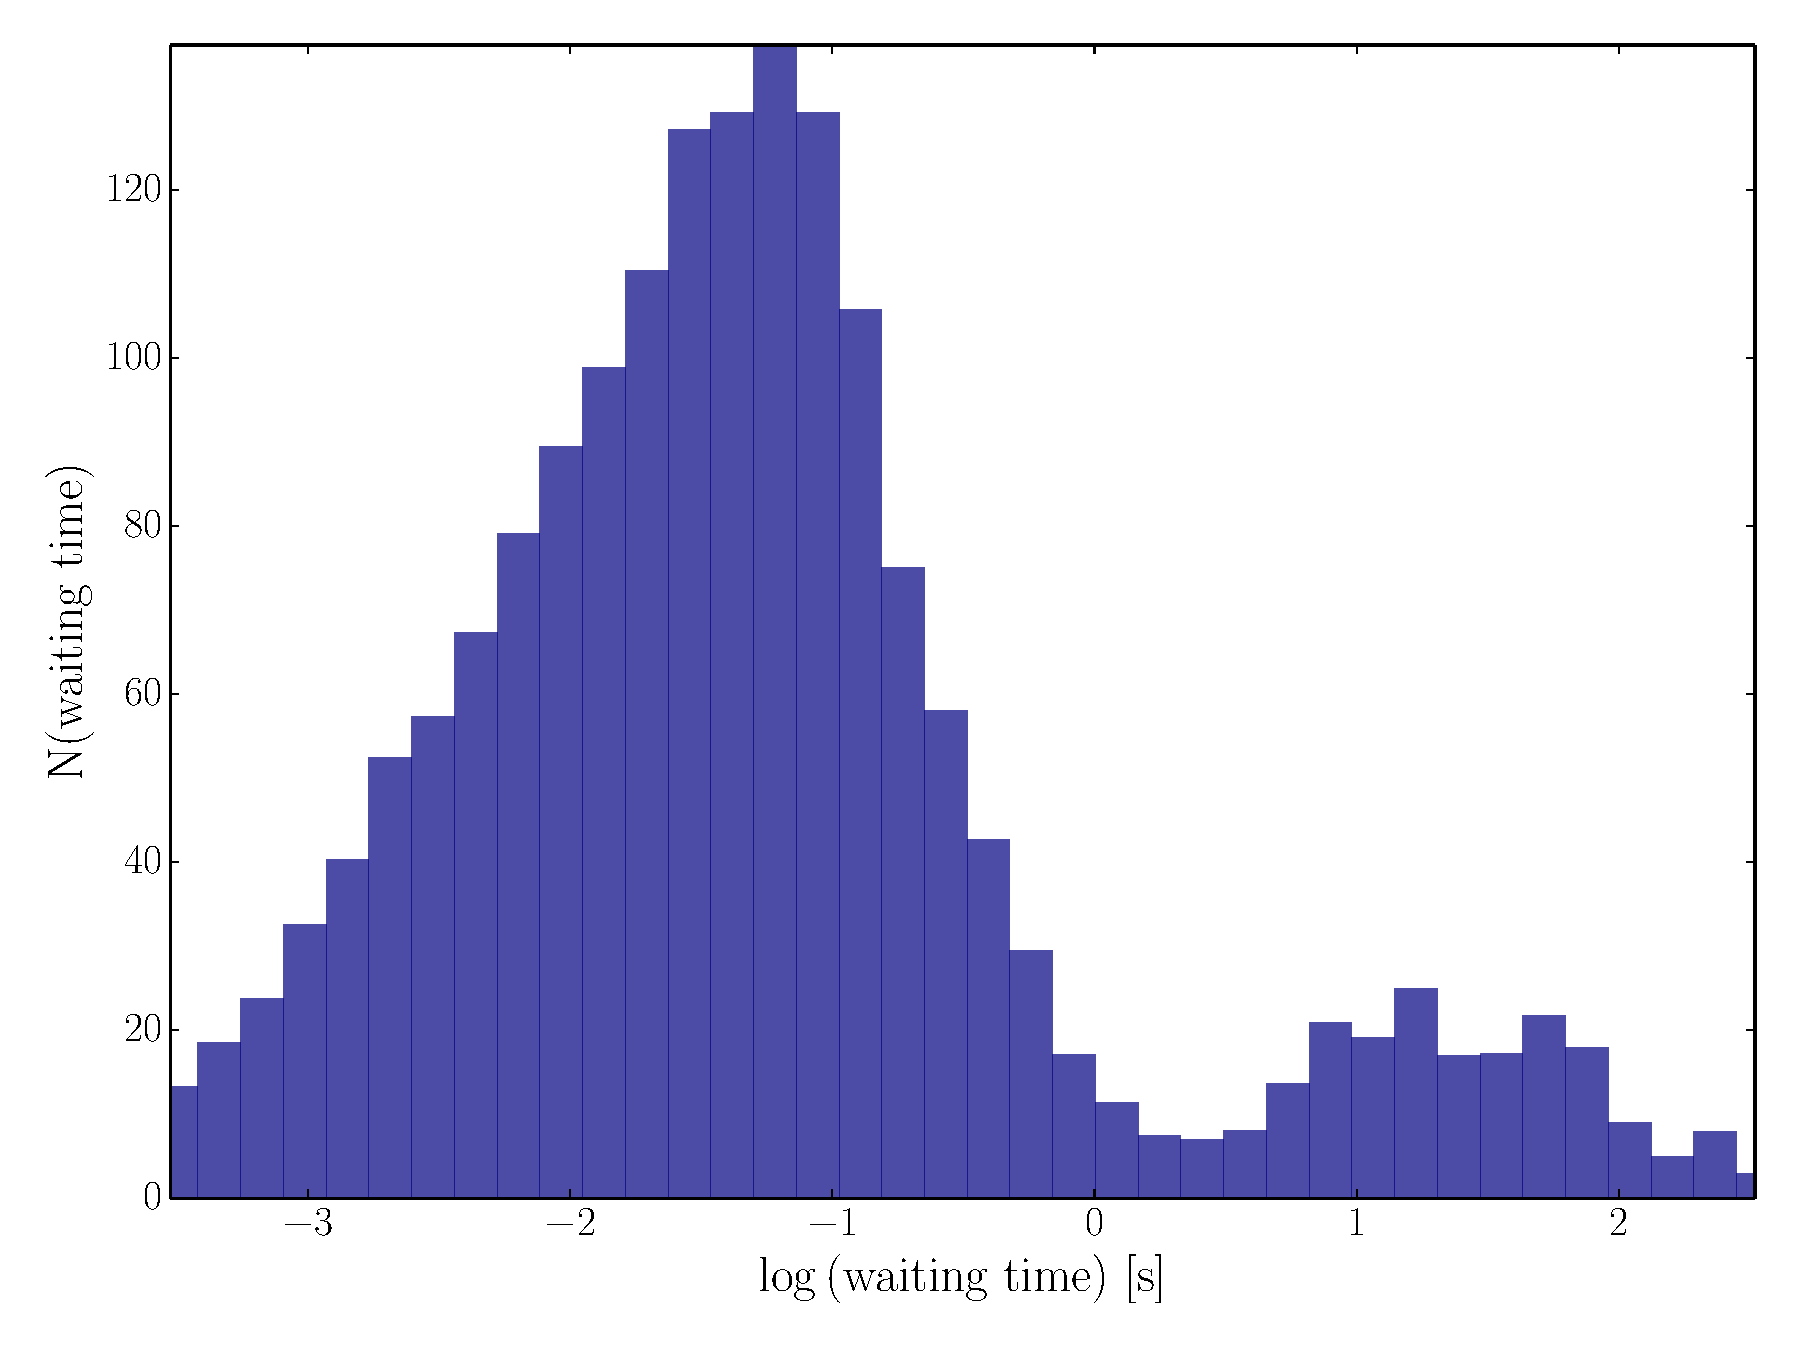
\includegraphics[width=9cm]{sgr1550_waitingtimes.pdf}
\caption{Waiting time distribution between consecutive spikes for $332$ bursts. Waiting times are the times between peak amplitudes of spikes, and are only computed for
continuous stretches of data between them, i.e. time series without data gaps. This effectively sets an upper limit to the waiting time that can be measured of $330\,\mathrm{s}$, the 
length of a single \fermi/GBM trigger.}
\label{fig:waitingtimes}
\end{center}
\end{figure}

In Figure \ref{fig:waitingtimes}, we show the differential distribution of waiting times for $332$ magnetar bursts. We use only waiting times 
between consecutive spikes that have no data gaps between them. This effectively sets an upper limit to the waiting time distribution of $330\,\mathrm{s}$,
the length of a single \fermi/GBM trigger. The distribution is clearly bimodal: a broad peak at long waiting times has a maximum at $\sim 20 \,\mathrm{s}$, a
second peak at smaller waiting times, $t_\mathrm{wait} \approx 0.05 \,\mathrm{s}$. This implies that there are two significantly different time scales
in the system, as expected. In our definition, bursts are clusters of individual peaks separated by
waiting times much longer than their durations. It is the time between these bursts that sets the peak in long waiting times. This distribution has a peak about
an order of magnitude lower than that reported for the strongest-field magnetars, SGR 1900+14 \citep{gogus1999} and SGR 1806-20 \citep{gogus2000} as observed
with \rxte, however, we note that the intrinsic short duration of \fermi/GBM observation imposes an artificial limit of $330\,\mathrm{s}$ on the waiting times we measure,
and thus likely introduces a significant bias towards short waiting times. 
The distribution of short waiting times, on the other hand, traces the time between consecutive spikes within a burst. The sharp peak of this distribution indicates
that there is a characteristic time scale determining the waiting time between individual peaks within a burst as well. 

 \begin{figure*}[htbp]
\begin{center}
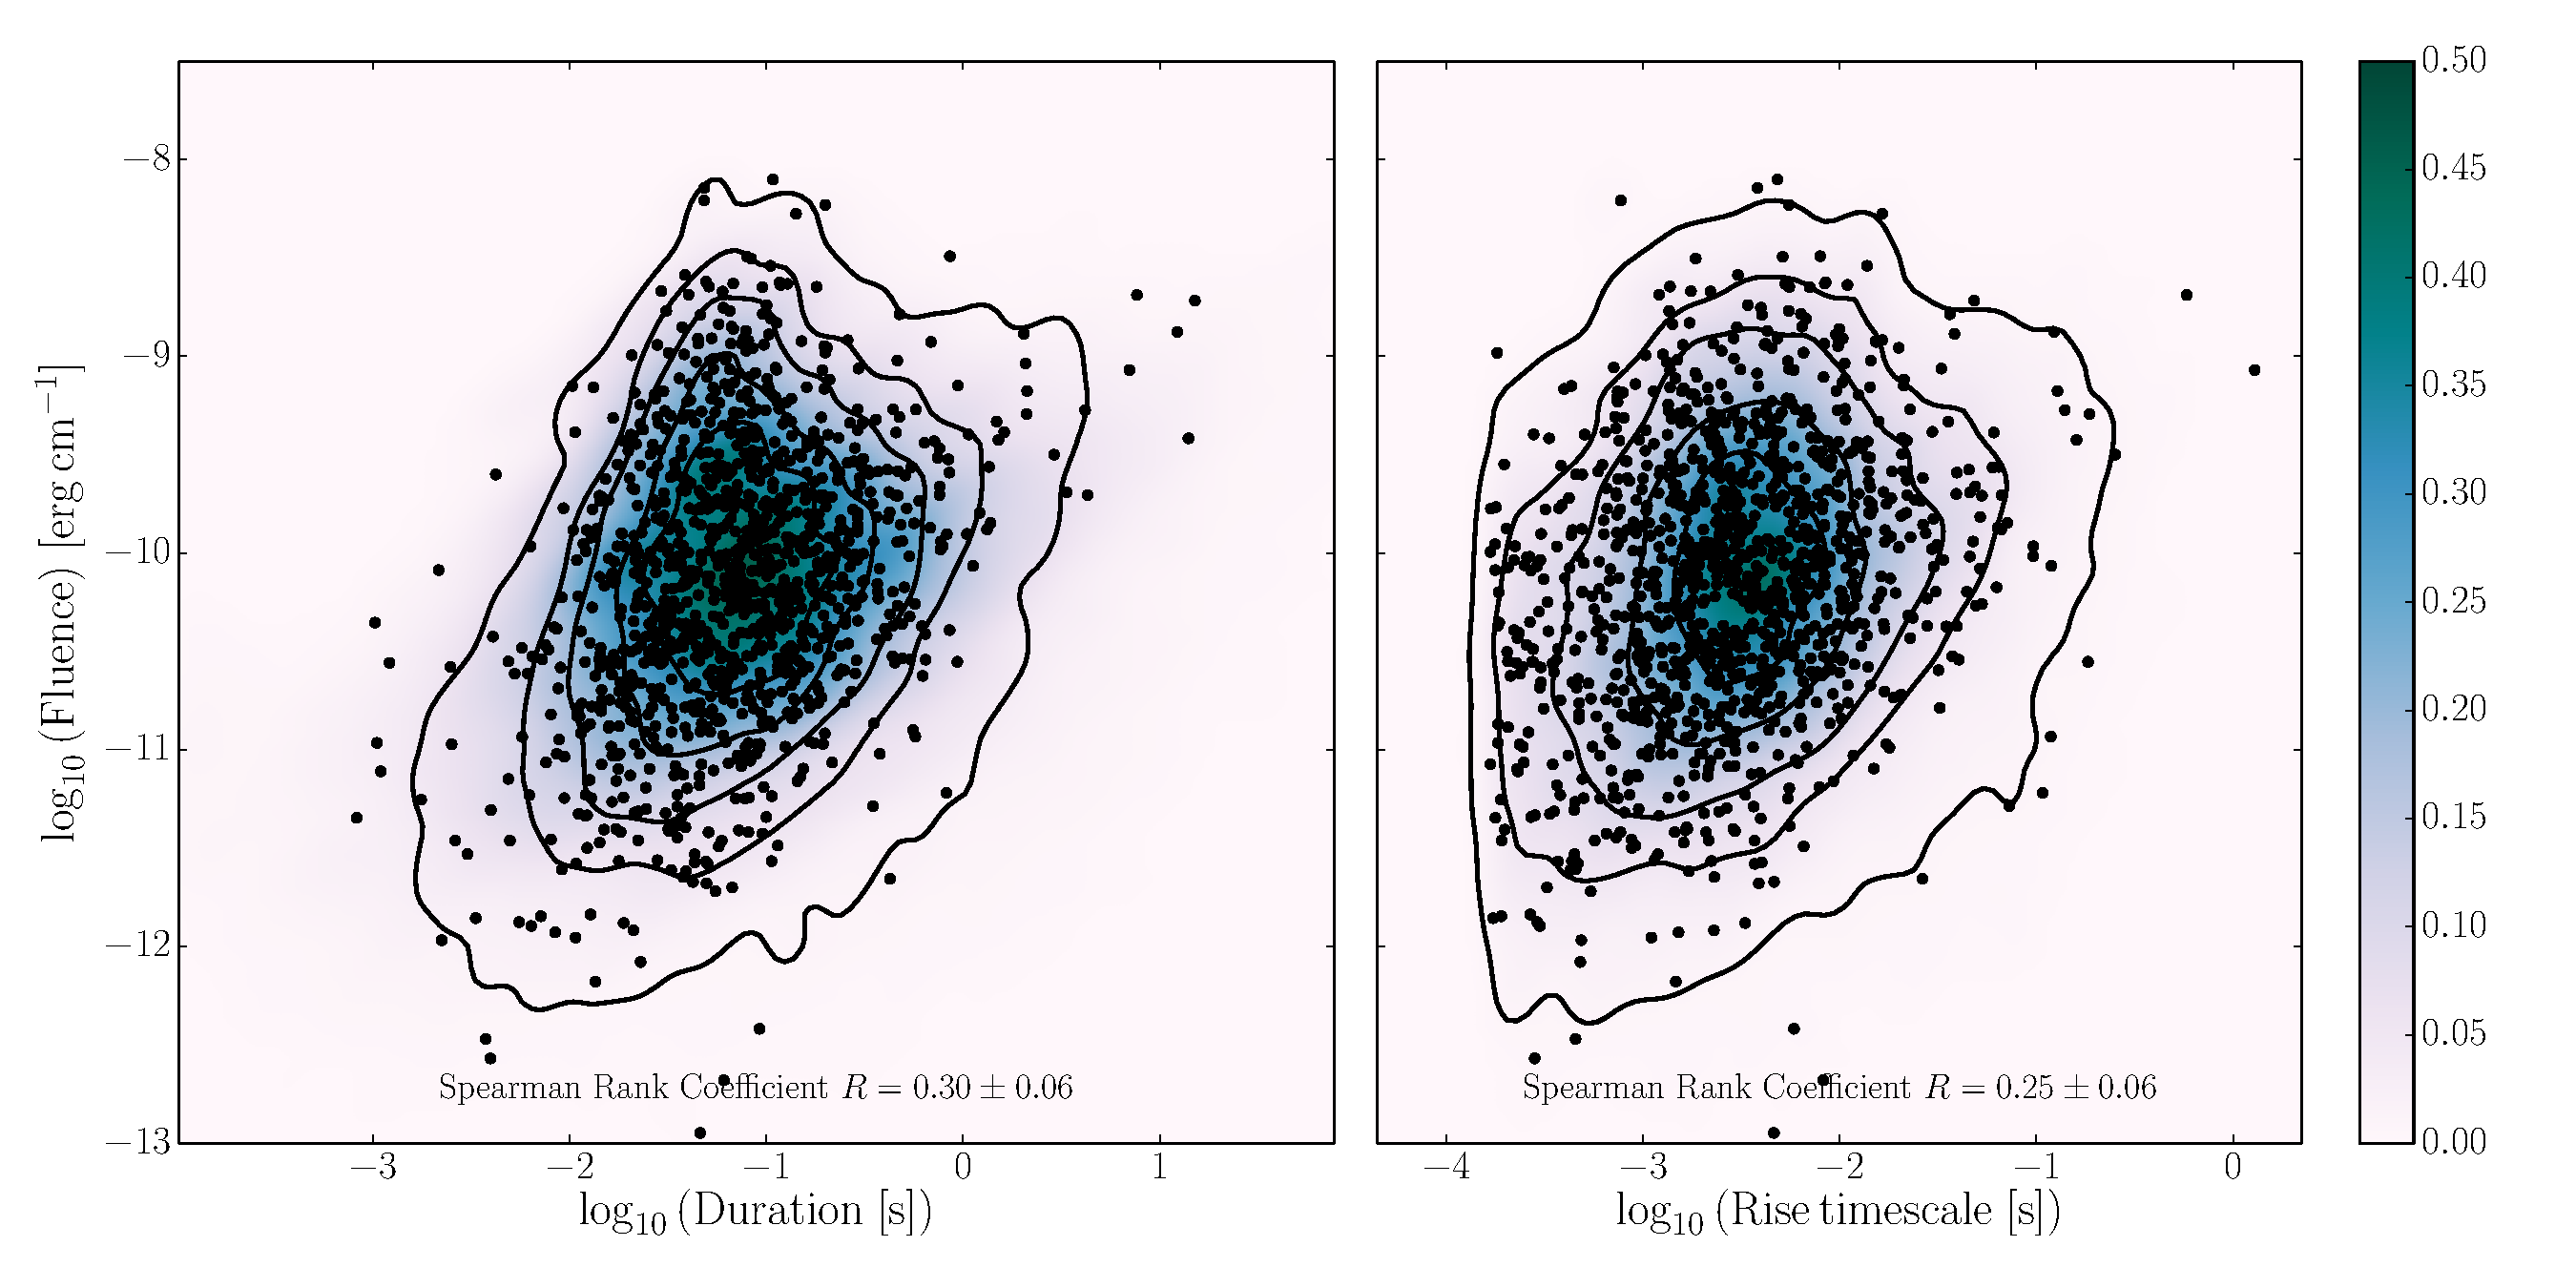
\includegraphics[width=\textwidth]{sgr1550_correlations.pdf}
\caption{Correlations between spike duration and fluence (left) and spike rise time and fluence (right). Black points indicate an ensemble of burst models, where we drew once
from the posterior pdf of each burst to build the ensemble. Contours are derived from the combined sample of $100$ draws for all bursts, the shaded background is constructed in
the same way for illustrative purposes. Contour levels are at $0.01, 0.05, 0.1, 0.2$ and $0.3$.
The duration is defined as the time between the two points where
the count rate drops to $0.01$ of the peak count rate on either side of that peak, computed from the inferred model parameters of each spike. The rise time is the exponential
rise time scale defined in Equation \ref{eqn:word}. The fluence is calculated by computing the fraction of the total number of bursts in a spike compared to the whole burst, and using
this fraction in combination with fluences inferred from spectral modelling\citep{vanderhorst2012,vonkienlin2012} to derive the fluence in a single spike.}
\label{fig:correlations}
\end{center}
\end{figure*}

In Figure \ref{fig:correlations}, we plot rise time and duration against fluence for all $332$ bursts. There is a clear positive
correlation between both rise time and fluence as well as spike duration and fluence (Spearman rank coefficient $R = 0.30\pm0.06$ with $p < 10^{-5}$ for duration versus fluence,
and $R = 0.25\pm0.06$ with $p < 0.01$ for duration versus rise time). Clearly, more energetic spikes require both more time to rise to the peak,
and radiate away their energy for a longer overall time. This is consistent with the results from \citep{gogus1999}, who found a correlation between
duration and fluence for bursts from SGR 1900+14, which could be modelled with a power law with an index of $1.13$. 

 \begin{figure}[htbp]
\begin{center}
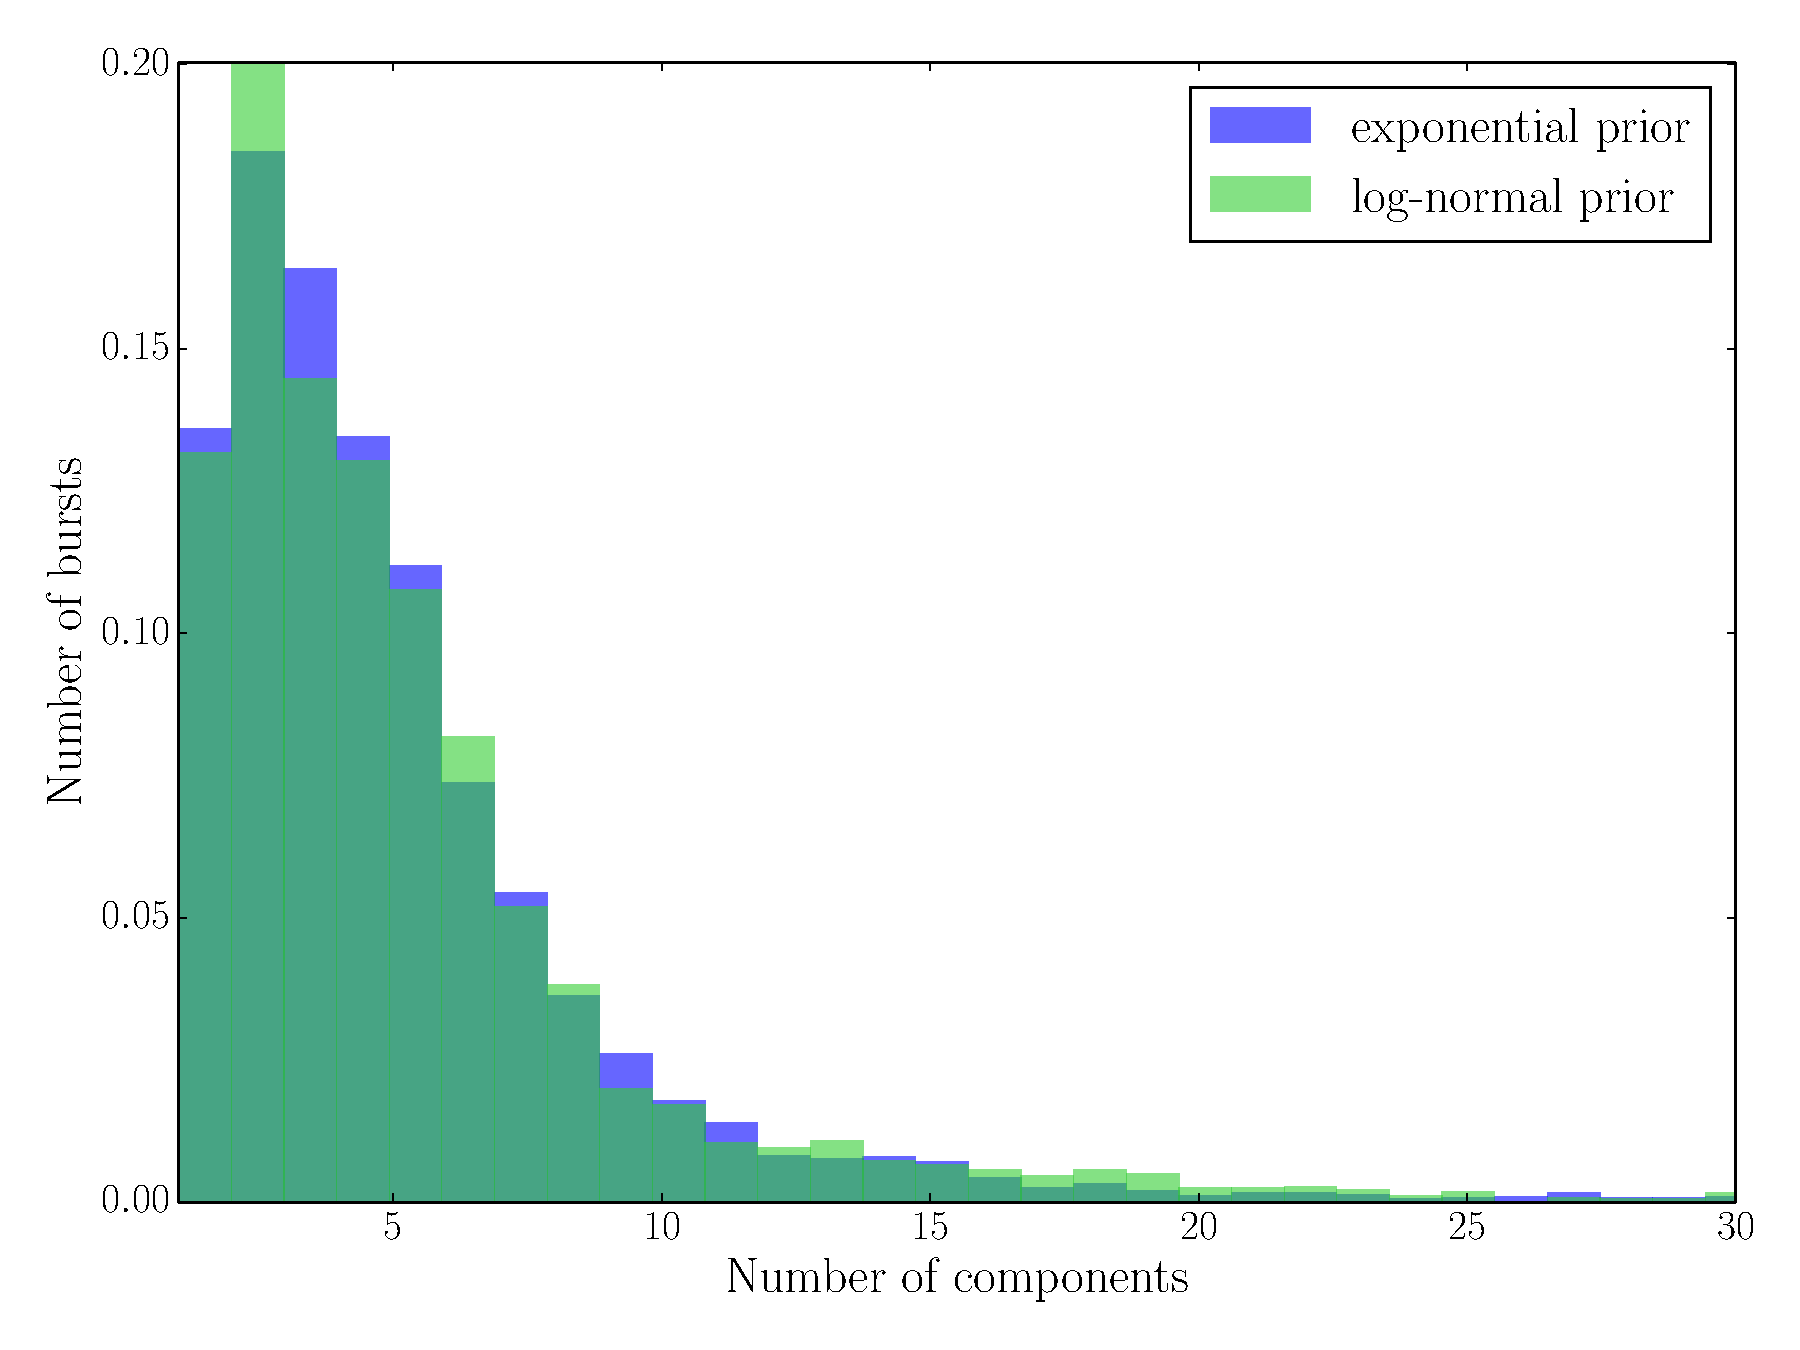
\includegraphics[width=9cm]{sgr1550_prior_nspikes.pdf}
\caption{The number of  components (spikes) per burst for $332$ bursts for both exponential priors (blue) for amplitude and rise time scale, the standard prior assumed in
deriving the results of this work, and log-normal priors (green) as an alternative hypothesis for the prior distributions on amplitude and rise time scale. Changing the prior has 
no appreciable effect on the number of components per burst.}
\label{fig:nspikes_prior}
\end{center}
\end{figure}

\begin{figure*}[htbp]
\begin{center}
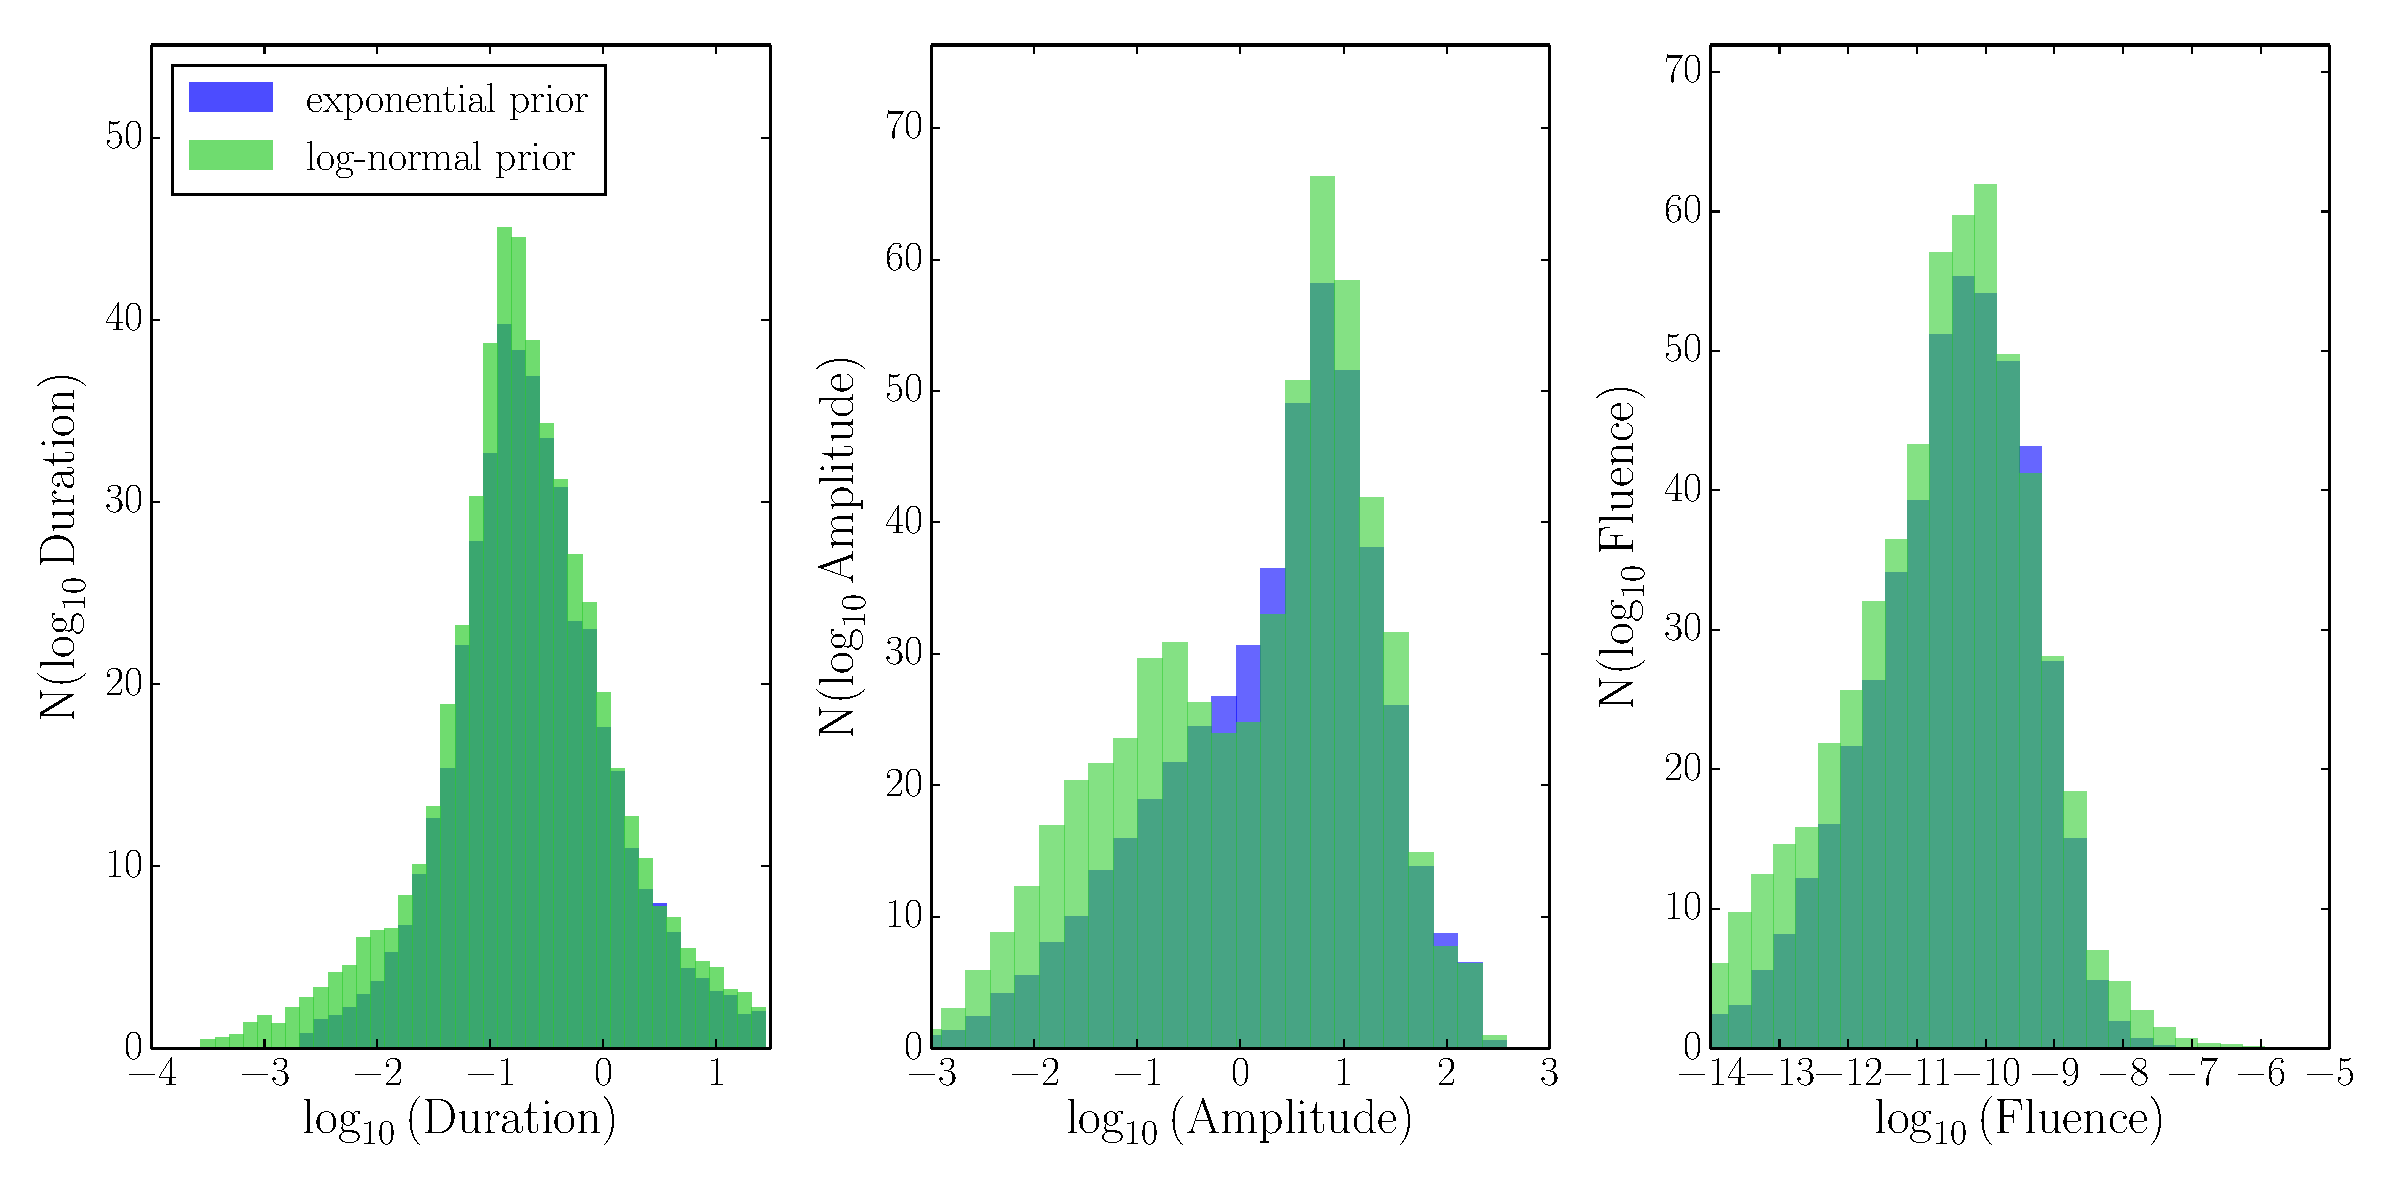
\includegraphics[width=\textwidth]{sgr1550_prior_diff_dist.pdf}
\caption{Differential distributions for burst duration (left panel), amplitude (middle panel) and fluence (right panel) for an exponential prior on spike 
amplitudes and rise timescales (blue; see also Figure \ref{fig:diffdist}),
and a log-normal prior on the same parameters (green). A log-normal prior leads to a noticeable increase in low-amplitude spikes (middle panel), translating
to an excess at low fluences as well. The overall shape and location of the maximum for each distribution, however, remains unchanged.}
\label{fig:diff_prior}
\end{center}
\end{figure*}
\subsection{Testing the Prior Assumptions}

Because we have little prior information about the nature of magnetar bursts and the details of
the underlying physical processes producing them, we choose mostly uninformative priors for all model parameters. However,
there is still some leeway in the choice of these prior distributions, and thus it merits investigation whether changing
any priors will have an appreciable impact on the conclusions we derive. 

The strongest source of uncertainty in terms of deriving conclusions from the data set comes from the priors for
amplitudes and rise time. An exponential distribution favours low-amplitude spikes with short rise time, which, in principle,
could give rise to a population of very short, very small spikes modelling individual photons in high-resolution light curves. We have already shown in 
Section \ref{sec:exploration} that the generally low number of components per burst disfavours this interpretation. In order
to improve our understanding how this prior could influence our results, we implemented a log-normal prior for both rise time
and amplitude, with the mean and standard deviations of each distribution free hyper parameters. Because of the use of improper priors
on the background parameter as well as the hyper parameter for the amplitude, we do not perform a formal model selection
(e.g. using the marginal likelihood introduced in Equation \ref{eqn:marginal}), but simply explore how the use of different priors
changes the results reported in the previous section.







In Figures \ref{fig:nspikes_prior} and \ref{fig:diff_prior} we present a comparison between the distributions for the number of spikes 
per burst from $82$ bursts for each set of priors, and the differential distributions for the most important quantities for both priors.
In both cases, we consider the full, unfiltered sample here, since it is the spikes with the smallest amplitudes where we expect to see
an appreciable difference. Overall, there is no significant difference in the number of components per burst, indicating that both 
priors lead to similar results. However, we do see an excess of small-amplitude spikes for a log-normal prior in the differential 
distributions for duration, amplitude, and, correspondingly, fluence. Using lognormal priors on the amplitude seems to increase
the probability of a model consisting of many low-amplitude spikes. Why exactly this should be the case is not immediately 
obvious and merits further exploration. However, given that the presence of these low-amplitude spikes is difficult to constrain no matter
the prior, and they do little to change our conclusions from the data, we defer this in-depth exploration of prior to future work.


\section{Discussion}


\subsection{Comparison with SOC Predictions}
\label{sec:soc}

Magnetar bursts have often been placed in the context of self-organised criticality (SOC). In this framework, a physical system continuously drives
itself towards a critical point, without fine tuning or outside intervention. When reaching this critical point, a catastrophic energy
release will return the system to a sub-critical state, upon which the cycle begins anew. The standard cellular automaton model of \citet{bak1987} models an SOC system as a grid of cells (or nodes), where activation of one node leads to a cascade of activation in neighbouring nodes based on some activation rule (e.g. a preferential direction), leading to 
sudden energy release and dissipation and return of the system to the sub-critical state.
Based on the avalanche evolution, it becomes possible to define a characteristic length scale and affected 
area (or volume) in the system, which is closely related with the released energy. 
The evolution of typical avalanche length scales follows a classical diffusion law, set by a diffusion coefficient $\beta$. 
 Using this diffusion law, it is possible to derive detailed predictions for the relationships between different quantities.

One of the defining features of the SOC framework is that while the details of the physical processes in question depend on the characteristics
of the system, SOC leads to an overall characteristic behaviour with similar statistical properties for many different systems. 


 This framework has been successfully employed to model, for example, solar flares \citep[for an overview see ][ and references therein]{aschwanden2014}.
In particular, the SOC framework makes predictions for power law-type correlations between various quantities - most importantly, duration, 
peak amplitude and total dissipated energy -  as well as their differential distributions. 
The predicted correlations for the avalanche duration $D$, peak flux $F$ and total dissipated energy $E$ are

\begin{eqnarray}
P & \propto  T^{d\beta/2} &\propto  T^{3/2} \\ 
E &\propto   T^{D_d\beta/2 + 1} & \propto  T^{2} \\
\end{eqnarray}

for typical values for the (mean) fractal dimension $D_d \approx (1+d)/2$, the spatial dimension $d = 3$ for Euclidean space, and a
classical diffusion coefficient  $\beta = 1$ \citep[see ][ and references therein for details of the derivation]{aschwanden2014}. 
As expected from SOC predictions, we see a positive correlation between spike duration and 
fluence (a proxy for the total dissipated energy), similar to that seen when taking the bursts as a whole \citep{gogus1999}. 
The slope of this correlation seems to be flatter than the $T^{2}$ proportionality
expected from classical SOC, although this requires confirmation with a hierarchical model that allows proper inference over many
bursts at the same time.  

The differential distributions of burst duration, peak amplitude and total dissipated energy can be derived as

\begin{eqnarray}
N(T) dT &=& T^{-\alpha_T}dT \;  \mbox{; $\alpha_T = 1 + (d-1)\frac{\beta}{2}$} = 2\nonumber \\ 
N(A) dA &=& T^{-\alpha_A}dA \; \mbox{; $\alpha_A = 2 - \frac{1}{d}$} = 5/3 \\
N(E) dE & = &T^{-\alpha_E}dE  \;\mbox{; $\alpha_E = 1 + \frac{(d-1)}{(D_d + 2/b)}$} =  3/2 \; ,  \nonumber
\end{eqnarray}

again for the standard assumptions stated above. Unlike the correlations between parameters, the differential
 distributions do not follow the expected power laws: all three quantities show strongly peaked, unimodal distributions.
 While some of that may be an artefact of excluding the weakest, unconstrained peaks (with amplitudes lower than the inferred
 background count rate) from the sample, this selection cannot account for the complete disparity between theoretical 
 expectations and the inferred distributions from the data. Especially the fluence distribution additionally also disagrees strongly
 with the derived differential fluence distributions when considering bursts as a whole, which is known to be power law-like over at least 
 four orders of magnitude \citep{gogus1999,gogus2000,prieskorn2012}.
 It is possible that there is a population of weak, low-amplitude peaks even beyond those predicted by the model considered 
 here that we cannot see due to instrumental and sky background.
Alternatively, if there truly is a paucity of peaks at low amplitudes, durations and energies, this would indicate that while bursts as a
whole behave as an SOC system, the driving process that produces the intra-burst variability does not.

The waiting time distribution for magnetar bursts has traditionally been modelled as a log-normal distribution, with limited knowledge 
in the tail on both sides due to two dominant factors. At long waiting times, a lack of continuous monitoring and the resulting data gaps
make an accurate determination of long waiting times problematic. At the short end, there is a fundamental uncertainty in the definition of 
a single burst (indeed, \citealp{gogus1999} and \citealp{gogus2000} do not model waiting times $<3\,\mathrm{s}$ in order to avoid confusion between 
separate, single-peaked bursts and multi-peaked bursts). 

In the SOC framework, the occurrence of individual avalanches is generally modelled as a random process: the distribution of critical events in time
follows a Poisson process. This process can either be stationary for a constant driving process, or more often the driving process setting the frequency
of burst occurrences is non-stationary in some way. The details of this non-stationarity will determine the shape of the resulting waiting time distribution.
However, even for a non-stationary Poisson process, the resulting waiting time distribution will be a superposition of two or more exponential distributions,
no matter the time-dependent behaviour of the underlying driving process. The resulting distribution 
can be approximated as a power law at long waiting times (see \citealp{aschwanden2011} for derivations for various driving processes), which flattens out at 
short waiting times. 

This is not what is observed when decomposing magnetar bursts into individual spike-like features (cf Figure \ref{fig:waitingtimes}. There is a
clear bimodality that is at odds with the power law-like predictions of SOC theory. Even for a driving process that operates at a low
rate for most of the time, and only occasionally drives a short period of intense avalanching, SOC predicts a power law that flattens at short
waiting times. Again, it may be possible to explain some of the discrepancy with a lack of well-constrained low-amplitude spikes hidden in 
the background, but this does not explain the clear bimodality between long and short waiting times. This may be an indicator that two different
processes, with two different characteristic time scales, operate in producing the bursts and the intra-burst variability, respectively. 


\subsection{Crust Fracture versus Explosive Reconnection}


\section{Conclusions}

- for the first time model magnetar light curve variability in a probabilistic (unbiased?) way \\
- proof of principle: can extract information relevant to physical processes in the system \\
- can in principle extract time scales and find correlations between parameters that may be
indicative of SOC processes \\
- need a *lot* more work on theory, both explosive reconnection and crust fracture processes \\
- this research supposed to be a stepping stone towards a better understanding, need to be
more driven by theoretical developments! \\
- future directions: hierarchical models for proper inference over many bursts, hierarchical inference
over different sources, testing priors + model shapes in a more rigorous way.


\paragraph{acknowledgements}
We thank the organizers of MaxEnt2013.


\bibliography{td}
\bibliographystyle{apj}

\end{document}
